% -*- Mode:TeX -*-

%% IMPORTANT: The official thesis specifications are available at:
%%            http://libraries.mit.edu/archives/thesis-specs/
%%
%%            Please verify your thesis' formatting and copyright
%%            assignment before submission.  If you notice any
%%            discrepancies between these templates and the 
%%            MIT Libraries' specs, please let us know
%%            by e-mailing thesis@mit.edu

%% The documentclass options along with the pagestyle can be used to generate
%% a technical report, a draft copy, or a regular thesis.  You may need to
%% re-specify the pagestyle after you \include  cover.tex.  For more
%% information, see the first few lines of mitthesis.cls. 

%\documentclass[12pt,vi,twoside]{mitthesis}
%%
%%  If you want your thesis copyright to you instead of MIT, use the
%%  ``vi'' option, as above.
%%
%\documentclass[12pt,twoside,leftblank]{mitthesis}
%%
%% If you want blank pages before new chapters to be labelled ``This
%% Page Intentionally Left Blank'', use the ``leftblank'' option, as
%% above. 

\documentclass[12pt,twoside]{mitthesis}
\usepackage{lgrind}
\usepackage{amsmath}
\usepackage[mathscr]{euscript}
\usepackage{graphicx,color,colortbl}
\usepackage{bm,amsfonts,graphics}
\usepackage{cleveref}

\newtheorem{theorem}{Theorem}
%% These have been added at the request of the MIT Libraries, because
%% some PDF conversions mess up the ligatures.  -LB, 1/22/2014
\usepackage{cmap}
\usepackage[T1]{fontenc}
\pagestyle{plain}

\graphicspath{{./}{figures/}}
%% This bit allows you to either specify only the files which you wish to
%% process, or `all' to process all files which you \include.
%% Krishna Sethuraman (1990).

% %\typein [\files]{Enter file names to process, (chap1,chap2 ...), or `all' to 
% %process all files:}
\def\files{all}
\def\all{all}
\ifx\files\all \typeout{Including all files.} \else \typeout{Including only \files.} \includeonly{\files} \fi

\begin{document}

\pagestyle{plain}
%% This is an example first chapter.  You should put chapter/appendix that you
%% write into a separate file, and add a line \include{yourfilename} to
%% main.tex, where `yourfilename.tex' is the name of the chapter/appendix file.
%% You can process specific files by typing their names in at the 
%% \files=
%% prompt when you run the file main.tex through LaTeX.
\chapter{Problem Definition for Pursuit-Evasion Games}

Pursuit-evasion problems involve two players controlling a dynamic system of the form: 
\begin{equation*}
x^{k+1}=f(x^k, u_1, u_2)
\end{equation*}
Where $x^k$ is the current state, $u_1$ is the control of the first player (called the pursuer), $u_2$ is the control of the second player (called the evader), and $x^{k+1}$ is the new state based on the previous state and the control of both players. Furthermore, each of the players have competing interests where they wish to move the state $x$ into mutually exclusive target regions $\mathscr{T}_1$ and $\mathscr{T}_2$ respectively. Because of this the pursuer and evader choose their strategies with accordance to some value function $V(x,u_1,u_2)$: 
\begin{eqnarray*}
u_1^* & = & \underset{u_1}{\operatorname{argmin}}V(x,u_1,u_2)\\
u_2^* & = & \underset{u_2}{\operatorname{argmax}}V(x,u_1,u_2).
\end{eqnarray*}
Often in pursuit-evasion games it is common to either set the state as the distance between the two players or to place some cost on the distance between the players. The pursuer then tries to reach the origin or point of lowest cost in the shortest amount of time, while the evader either prolongs the state reaching this point for the longest amount of time or escapes the pursuer by increasing the distance to some specified value or reaching an escape region. Due to the nature that each player improves their cost by making an equal detriment to the cost of the other player, pursuit-evasion games are often modeled as zero-sum games. In games of this type, there exists a single cost function $G(x)$ where one player tries to maximize this function while the other player attempts to minimize it. This problem can also be modeled where each player tries to maximize or minimize their own cost function which is the negative of the opposing player's cost function $(G_1(x) = -G_2(x))$.

Using this definition of pursuit-evasion games, in this paper I attempt to solve two games of this type. First I attempt to solve a four-dimensional game that can be solved without the help of tensor-train decomposition. Next I attempt to solve a six-dimensional game that is efficiently solved with the assistance of tensor-train decomposition.

One method of solving pursuit-evasion games is to use dynamic programming. This method attempts to solve control problems by providing a value for each state in a discretized state space. Given that the states are discretized to a resolution $h$, where the discrete states are ${z_i:z_i \in l}$ and $l$ is the continuous state space, a stochastic optimal control problem can be solved using value iteration and the update function:
\begin{equation}\label{eqn8}
J^{k+1}(z_i)= \underset{u }{\operatorname{min }}[G(z_i,u) + \gamma \sum_{j}P(z_j|z_i, u)J^{(k)}(z_j)],
\end{equation}
in which $\gamma$ is the discount rate that ranges from $(0,1)$. $J^{(k)}$ will converge to the optimal cost-to-go function as $k \rightarrow \infty$ giving the Bellman equation:
\begin{equation*}
J^*(z_i) = \underset{u }{\operatorname{min }}[G(z_i,u) + \gamma \sum_{j}P(z_j|z_i,u)J^*(z_j)].
\end{equation*}  


Tensor-train value iteration can be modified to solve pursuit-evasion games using a best response dynamic. Instead of using a single update function as in \ref{eqn8}, I model the problem as solving two separate update functions over the same state-space:

\begin{equation}\label{eqn10}
\overline{J}^{(k+1,K)}(z_i)= \underset{u_1 }{\operatorname{min }}[G(z_i,u_1,u_2)+\gamma \sum_{j} P(z_j|z_i,u_1,u_2) J^{(k,K)}(z_j)],
\end{equation}
\begin{equation}\label{eqn11}
\underline{J}^{(k+1,K)}(z_i)= \underset{u_2 }{\operatorname{max }}[G(z_i,u_1,u_2)+\gamma \sum_{j} P(z_j|z_i,u_1,u_2) J^{(k,K)}(z_j)],
\end{equation}
By setting the opposing players' strategies to some constant strategy, I can run tensor-based value iteration on each of the optimization problems and solve for the optimal strategy of each of the players: $u_{1}^{*,1}$ and $u_{2}^{*,1}$ respectively. After solving for the optimal strategy for each of the players, I replace the constant strategy with the calculated optimal strategy. Given that for iteration $K$, the optimal strategy for each of the players is $u_{1}^{*,K}$ and $u_{2}^{*,K}$ respectively. If $u_{1}^{*,K}$ and $u_{2}^{*,K}$ each converge to a single strategy as $K \rightarrow \infty$, then by best response $u_{1}^{*,\infty}$ and $u_{2}^{*,\infty}$ are the optimal strategies for each of the players \cite{fuden}.

 

\section{Four-Dimensional Problem}
For the simple four dimensional problem, I have modeled a pursuer and evader in a $10 \times 10$ two-dimensional  state space with simple Euclidean dynamics. The four dimensions are the $x$ position of the pursuer $x_1$, the $y$ position of the pursuer $y_1$, the $x$ position of the evader $x_2$, and the $y$ position of the evader $y_2$. Each of the dimensions are bounded as follows:
\begin{eqnarray*}
x_1 & \in & [0,10]\\
y_1 & \in & [0,10]\\
x_2 & \in & [0,10]\\
y_2 & \in & [0,10].
\end{eqnarray*} 
Both the pursuer and the evader have two controls for their $x$ and $y$ velocity respectively, $u_1 = (Vx_1,Vy_1)$ and $u_2 = (Vx_2,Vy_2)$. These velocities are also bounded:
\begin{eqnarray*}
Vx_1 & \in & [-1,1]\\
Vy_1 & \in & [-1,1]\\
Vx_2 & \in & [-0.5,0.5]\\
Vy_2 & \in & [-0.5,0.5].
\end{eqnarray*} 
Furthermore, the following system dynamics are used:
\begin{eqnarray}\label{eqns1}
x_1^{k+1} & = & x_1^k +Vx_1dt,\\
y_1^{k+1} & = & y_1^k +Vy_1dt,\\
x_2^{k+1} & = & x_2^k +Vx_2dt,\\
y^{k+1}_2 & = & y_2^k +Vy_2dt.
\end{eqnarray}
Each dimension is discretized into 21 equally spaced states for a total of $21^4 \approx 2\cdot10^5$ discrete states. This discretization was chosen as it creates a state for every $0.5$ units:
\begin{eqnarray*}
x_1 & \in & \left\{0,0.5,1,1.5,2,2.5,3,3.5,4,4.5,5,5.5,6,6.5,7,7.5,8,8.5,9,9.5,10\right\}\\
y_1 & \in & \left\{0,0.5,1,1.5,2,2.5,3,3.5,4,4.5,5,5.5,6,6.5,7,7.5,8,8.5,9,9.5,10\right\}\\
x_2 & \in & \left\{0,0.5,1,1.5,2,2.5,3,3.5,4,4.5,5,5.5,6,6.5,7,7.5,8,8.5,9,9.5,10\right\}\\
y_2 & \in & \left\{0,0.5,1,1.5,2,2.5,3,3.5,4,4.5,5,5.5,6,6.5,7,7.5,8,8.5,9,9.5,10\right\}.
\end{eqnarray*} 
 
Value iteration can be used to solve for the optimal cost at each state. The problem is modeled as a discounted, deterministic, shortest path problem where $\gamma = 0.7$ and $P(z_j|z_i,u_1,u_2) = 1$ where $z_j$ is the deterministic result of $f(z_i,u_1,u_2)$. Each iteration of best response $K$ results in an optimal control policy which is used as a constant control policy for the opponent. Given an initial condition $z_i$, the optimal value can be solved for the pursuer or evader by using the following update functions respectively:
\begin{equation}\label{4pbell}
J^{(k+1,K)}(z_i)= \underset{u_1 }{\operatorname{min }}[10+(x_1-x_2)^2+(y_1-y_2)^2+0.7 J^{(k,K)}(z_j|z_i,u_1,u_2^K)],
\end{equation}
\begin{equation}\label{4ebell}
J^{(k+1,K)}(z_i)= \underset{u_2 }{\operatorname{max }}[10+(x_1-x_2)^2+(y_1-y_2)^2+0.7 J^{(k,K)}(z_j|z_i,u_1^K,u_2)].
\end{equation} 
By running the update functions until $k \rightarrow \infty$, the optimal value function is achieved for a given opponents control policy $u^K$:
\begin{equation}\label{4popt}
J^{(*,K)}(z_i)= \underset{u_1 }{\operatorname{min }}[10+(x_1-x_2)^2+(y_1-y_2)^2+0.7 J^{(*,K)}(z_j|z_i,u_1,u_2^K)],
\end{equation}
\begin{equation}\label{4eopt}
J^{(*,K)}(z_i)= \underset{u_2 }{\operatorname{max }}[10+(x_1-x_2)^2+(y_1-y_2)^2+0.7 J^{(*,K)}(z_j|z_i,u_1^K,u_2)].
\end{equation}
The optimal value functions can then be used to solve for the optimal control values $u_1^{(*,K)}$ and $u_2^{(*,K)}$:
\begin{equation}\label{4pcont}
u_1^{(*,K)}(z_i)= \underset{u_1 }{\operatorname{arg min }}[10+(x_1-x_2)^2+(y_1-y_2)^2+0.7 J^{(*,K)}(z_j|z_i,u_1,u_2^K)],
\end{equation}
\begin{equation}\label{4econt}
u_2^{(*,K)}(z_i)= \underset{u_2 }{\operatorname{arg max }}[10+(x_1-x_2)^2+(y_1-y_2)^2+0.7 J^{(*,K)}(z_j|z_i,u_1^K,u_2)].
\end{equation}

Furthermore if each iteration of best response is run until $K \rightarrow \infty$ and $u_1^{(*,K)}$ and $u_2^{(*,K)}$ each converge to a single set of control values, then those control values are considered a Nash equilibrium and:
\begin{equation}\label{4pbropt}
J^{(*,*)}(z_i)= \underset{u_1 }{\operatorname{min }}[10+(x_1-x_2)^2+(y_1-y_2)^2+0.7 J^{(*,*)}(z_j|z_i,u_1,u_2^*)],
\end{equation}
\begin{equation}\label{4ebropt}
J^{(*,*)}(z_i)= \underset{u_2 }{\operatorname{max }}[10+(x_1-x_2)^2+(y_1-y_2)^2+0.7 J^{(*,*)}(z_j|z_i,u_1^*,u_2)].
\end{equation}
The optimal control values can be determined by:
\begin{equation}\label{4pbrcont}
u_1^{(*,*)}(z_i)= \underset{u_1 }{\operatorname{arg min }}[10+(x_1-x_2)^2+(y_1-y_2)^2+0.7 J^{(*,*)}(z_j|z_i,u_1,u_2^*)],
\end{equation}
\begin{equation}\label{4ebrcont}
u_2^{(*,*)}(z_i)= \underset{u_2 }{\operatorname{arg max }}[10+(x_1-x_2)^2+(y_1-y_2)^2+0.7 J^{(*,*)}(z_j|z_i,u_1^*,u_2)].
\end{equation}    
These optimal value functions \ref{4pbropt} \ref{4ebropt} can be used to solve the following pursuit-evasion optimization problem:
\begin{eqnarray}\label{4opt}
&&\underset{u_1 }{\operatorname{min }}\underset{u_2 }{\operatorname{max }}[\int_{0}^{T}e^{-0.7t}(10+(x_1(t)-x_2(t))^2+(y_1(t)-y_2(t))^2)dt]\\
&\textnormal{s.t.}&\ref{eqns1}.
\end{eqnarray}
The problem also has a simple analytic solution since the dimensions are separable. For the pursuer, the optimal solution is:
\begin{equation}\label{puroptx}
Vx_1^*= \underset{Vx_1 }{\operatorname{arg min }}[((x_1 + Vx_1dt)-(x_2+Vx_2dt))^2],
\end{equation}
\begin{equation}\label{puropty}
Vy_1^*= \underset{Vy_1 }{\operatorname{arg min }}[((y_1 + Vy_1dt)-(y_2+Vy_2dt))^2].
\end{equation}
The optimal solution for the evader is then:
\begin{equation}\label{evadoptx}
Vx_2^*= \underset{Vx_2 }{\operatorname{arg max }}[((x_1 + Vx_1dt)-(x_2+Vx_2dt))^2],
\end{equation}
\begin{equation}\label{evadopty}
Vy_2^*= \underset{Vy_2 }{\operatorname{arg max }}[((y_1 + Vy_1dt)-(y_2+Vy_2dt))^2].
\end{equation}

The size of the state space allows this problem to be solved by both traditional value iteration and TTVI. First the problem was solved with the traditional value iteration algorithm. In order to implement the best response dynamic, the pursuer algorithm \ref{4pbell} was run for a hundred iterations with a constant evader strategy of $(Vx_2 = 0,Vy_2 = 0)$ for all states resulting in a state cost of $J^{(*,1)}_p$. It can be seen in \Cref{VIpursplot1,VIpursplot2,VIpursplot3,VIpursplot4,VIpursplot5,VIpursplot6,VIpursplot7,VIpursplot8} that the pursuer captures the stationary evader from a number of varying starting positions. \Cref{VIpursue0,VIpursue10,VIpursue98,VIpursue99} also show that the algorithm converges to the optimal state costs. Then the evader algorithm \ref{4ebell} was run for a hundred iterations with a constant pursuer strategy of $(Vx_1 = 0,Vy_1 = 0)$ for all states. This resulted in a state cost of $J^{(*,1)}_e$. \Cref{VIevadplot1,VIevadplot2,VIevadplot3,VIevadplot4,VIevadplot5,VIevadplot6,VIevadplot7,VIevadplot8} show that the evader maximizes its distance from the pursuer for a variety of pursuer starting positions. Convergence of the optimal state costs for the evader can also be seen in \Cref{VIevade0,VIevade10,VIevade98,VIevade99}. Next the pursuer algorithm \ref{4pbell} was run for a hundred iterations with the evader strategy produced from $J^{(*,1)}_e$ according to equation \ref{4econt}. $J^{(*,1)}_p$ was used as the starting state cost and the run resulted in the costs $J^{(*,2)}_p$. Now \Cref{VIpursbr1plot1,VIpursbr1plot2,VIpursbr1plot3,VIpursbr1plot4,VIpursbr1plot5,VIpursbr1plot6,VIpursbr1plot7,VIpursbr1plot8} show that the pursuer captures the moving evader from a variety of starting positions. \Cref{VIpursue1br0,VIpursue1br10,VIpursue1br98,VIpursue1br99} continue to show convergence of the function for the given evader control policy. The evader algorithm \ref{4ebell} was also run for a hundred iterations with the evader strategy produced from $J^{(*,2)}_p$ according to equation \ref{4pcont}.$J^{(*,1)}_e$ was used as the starting state cost and the run resulted in the costs $J^{(*,2)}_e$. \Cref{VIevadbrplot1,VIevadbrplot2,VIevadbrplot3,VIevadbrplot4,VIevadbrplot5,VIevadbrplot6,VIevadbrplot7,VIevadbrplot8} show that the evader delays the pursuer from gaining capture for a variety of pursuer starting positions. \Cref{VIevadebr0,VIevadebr10,VIevadebr98,VIevadebr99} continue to show convergence of the function for the given pursuer control policy.Finally the pursuer algorithm \ref{4pbell} was run a second time for a hundred iterations with the evader strategy produced from $J^{(*,2)}_e$ according to equation \ref{4econt}. $J^{(*,2)}_p$ was used as the starting state cost and the run resulted in the costs $J^{(*,3)}_p$. \Cref{VIpursbr2plot1,VIpursbr2plot2,VIpursbr2plot3,VIpursbr2plot4,VIpursbr2plot5,VIpursbr2plot6,VIpursbr2plot7,VIpursbr2plot8} show that the pursuer captures the moving evader from a variety of starting positions in the same manner as the pursuer in \Cref{VIevadbrplot1,VIevadbrplot2,VIevadbrplot3,VIevadbrplot4,VIevadbrplot5,VIevadbrplot6,VIevadbrplot7,VIevadbrplot8}. The control policy as demonstrated in \Cref{VIpursbr2plot1,VIpursbr2plot2,VIpursbr2plot3,VIpursbr2plot4,VIpursbr2plot5,VIpursbr2plot6,VIpursbr2plot7,VIpursbr2plot8} also matches the control policy gained from the analytic solution to the problem in \ref{puroptx},\ref{puropty},\ref{evadoptx}, and \ref{evadopty}. \Cref{VIpursue2br0,VIpursue2br99} remain unchanged from \Cref{VIpursue1br0,VIpursue1br10,VIpursue1br98,VIpursue1br99} showing that the pursuer state costs have converged to optimality.

Tensor-Train Value Iteration can also be used to solve the pursuit-evasion game with simple Euclidean dynamics. Once again the same five algorithm runs were used to demonstrate that the state costs converge to an optimal best response solution. All Tensor-Train Value Iteration runs were run with an error bounds of $1 \times 10^{-2}$. First, the pursuer algorithm \ref{4pbell} was run for a hundred iterations with a constant evader strategy of $(Vx_2 = 0,Vy_2 = 0)$ for all states resulting in a state cost of $J^{(*,1)}_p$. It can be seen in \Cref{TTVIpursplot1,TTVIpursplot2,TTVIpursplot3,TTVIpursplot4,TTVIpursplot5,TTVIpursplot6,TTVIpursplot7,TTVIpursplot8} that the pursuer captures the stationary evader from a number of varying starting positions. These figures also match those for the traditional value iteration in \Cref{VIpursplot1,VIpursplot2,VIpursplot3,VIpursplot4,VIpursplot5,VIpursplot6,VIpursplot7,VIpursplot8}. \Cref{TTVIpursue0,TTVIpursue10,TTVIpursue98,TTVIpursue99} also show that the algorithm converges to the optimal state costs within the error bounds. Next the evader algorithm \ref{4ebell} was run for a hundred iterations with a constant pursuer strategy of $(Vx_1 = 0,Vy_1 = 0)$ for all states. This again resulted in a state cost of $J^{(*,1)}_e$. \Cref{TTVIevadplot1,TTVIevadplot2,TTVIevadplot3,TTVIevadplot4,TTVIevadplot5,TTVIevadplot6,TTVIevadplot7,TTVIevadplot8} show that the evader maximizes its distance from the pursuer for a variety of pursuer starting positions. These figures also match those for the traditional value iteration in \Cref{VIevadplot1,VIevadplot2,VIevadplot3,VIevadplot4,VIevadplot5,VIevadplot6,VIevadplot7,VIevadplot8}. Convergence of the optimal state costs for the evader within error bounds can also be seen in \Cref{TTVIevade0,TTVIevade10,TTVIevade98,TTVIevade99}. The pursuer algorithm \ref{4pbell} was run again for a hundred iterations with the evader strategy produced from $J^{(*,1)}_e$ according to equation \ref{4econt}. $J^{(*,1)}_p$ was used as the starting state cost and the run resulted in the costs $J^{(*,2)}_p$. Now \Cref{TTVIpursbr1plot1,TTVIpursbr1plot2,TTVIpursbr1plot3,TTVIpursbr1plot4,TTVIpursbr1plot5,TTVIpursbr1plot6,TTVIpursbr1plot7,TTVIpursbr1plot8} show that the pursuer captures the moving evader from a variety of starting positions. \Cref{TTVIpursue1br0,TTVIpursue1br10,TTVIpursue1br98,TTVIpursue1br99} continue to show convergence of the function for the given evader control policy within error bounds. The evader algorithm \ref{4ebell} was also run again for a hundred iterations with the evader strategy produced from $J^{(*,2)}_p$ according to equation \ref{4pcont}.$J^{(*,1)}_e$ was used as the starting state cost and the run resulted in the costs $J^{(*,2)}_e$. \Cref{TTVIevadbrplot1,TTVIevadbrplot2,TTVIevadbrplot3,TTVIevadbrplot4,TTVIevadbrplot5,TTVIevadbrplot6,TTVIevadbrplot7,TTVIevadbrplot8} show that the evader delays the pursuer from gaining capture for a variety of pursuer starting positions. \Cref{TTVIevadebr0,TTVIevadebr10,TTVIevadebr98,TTVIevadebr99} continue to show convergence within error bounds of the function for the given pursuer control policy.Finally, the pursuer algorithm \ref{4pbell} was run a second time for a hundred iterations with the evader strategy produced from $J^{(*,2)}_e$ according to equation \ref{4econt}. $J^{(*,2)}_p$ was used as the starting state cost and the run resulted in the costs $J^{(*,3)}_p$. \Cref{TTVIpursbr2plot1,TTVIpursbr2plot2,TTVIpursbr2plot3,TTVIpursbr2plot4,TTVIpursbr2plot5,TTVIpursbr2plot6,TTVIpursbr2plot7,TTVIpursbr2plot8} show that the pursuer captures the moving evader from a variety of starting positions in much the same manner as the pursuer in \Cref{VIpursbr2plot1,VIpursbr2plot2,VIpursbr2plot3,VIpursbr2plot4,VIpursbr2plot5,VIpursbr2plot6,VIpursbr2plot7,VIpursbr2plot8}. The control policy as demonstrated in \Cref{TTVIpursbr2plot1,TTVIpursbr2plot2,TTVIpursbr2plot3,TTVIpursbr2plot4,TTVIpursbr2plot5,TTVIpursbr2plot6,TTVIpursbr2plot7,TTVIpursbr2plot8} also matches the control policy gained from the analytic solution to the problem in \ref{puroptx},\ref{puropty},\ref{evadoptx}, and \ref{evadopty}. \Cref{TTVIpursue2br0,TTVIpursue2br99} remain the same as \Cref{TTVIpursue1br0,TTVIpursue1br10,TTVIpursue1br98,TTVIpursue1br99} within error bounds showing that the pursuer state costs have converged to optimality. \Cref{TTVIpursbr2relplot} demonstrates that the relative $x$ and $y$ position between the pursuer and evader constantly decreases in an optimal fashion. \Cref{TTVIpursbr2phaseplot} shows the pursuer and evader positions with a one time step interval to better demonstrate the position of the pursuer and evader over time.

Both traditional value iteration and tensor-train value iteration can be used to solve the four-dimensional simple euclidean dynamics problem, however each method has its advantages and drawbacks. As seen in the state space costs in \Cref{VIpursue0,VIpursue10,VIpursue98,VIpursue99,VIevade0,VIevade10,VIevade98,VIevade99,VIpursue1br0,VIpursue1br10,VIpursue1br98,VIpursue1br99,VIevadebr0,VIevadebr10,VIevadebr98,VIevadebr99,VIpursue2br0,VIpursue2br99} for traditional value iteration and \Cref{TTVIpursue0,TTVIpursue10,TTVIpursue98,TTVIpursue99,TTVIevade0,TTVIevade10,TTVIevade98,TTVIevade99,TTVIpursue1br0,TTVIpursue1br10,TTVIpursue1br98,TTVIpursue1br99,TTVIevadebr0,TTVIevadebr10,TTVIevadebr98,TTVIevadebr99,TTVIpursue2br0,TTVIpursue2br99} for TTVI, the former converge to an exact value while the latter only converge within some error bounds. However, TTVI can tighten these error bounds at the potential increase in run time. Using the $1 \times 10^{-2}$ error bounds, TTVI runs approximately ten times faster than the traditional method as can be seen in \Cref{4dVIrt,4dTTVIrt}. Use of the TTVI algorithm also conserves memory. As seen in \Cref{4dstore}, the state cost representations of TTVI are approximately an eight the size of the four-dimensional arrays used to store the state costs in traditional value iteration. TTVI also allows for an increase in the discretization of the state space with modest computational time increases as seen in \Cref{4dTTVIrte}. This is in large part a result of the consistency of the tensor rank despite increases in state size. This four-dimensional example shows that TTVI provides many benefits for problems already solvable by traditional value iteration.               


\section{Six-Dimensional Problem}
For the six dimensional problem, the pursuer and evader adapt Dubins car dynamics as outlined in \cite{dubins}.  The pursuer and evader remain in a $10 \times 10$ two-dimensional  state space with the addition of a heading state for both. The six dimensions are the $x$ position of the pursuer $x_1$, the $y$ position of the pursuer $y_1$, the heading of the pursuer $\theta_1$, the $x$ position of the evader $x_2$, the $y$ position of the evader $y_2$, and the heading of the evader $\theta_2$. Each of the dimensions are bounded as follows:
\begin{eqnarray*}
x_1 & \in & [0,10]\\
y_1 & \in & [0,10]\\
\theta_1 & \in & [0,2\pi]\\
x_2 & \in & [0,10]\\
y_2 & \in & [0,10]\\
\theta_2 & \in & [0,2\pi].
\end{eqnarray*} 
Both the pursuer and the evader have a single control for their change in heading, respectively $u_1$ and $u_2$. These controls are bounded between $[-\dfrac{\pi}{4},\dfrac{\pi}{4}]$. The pursuer and evader each have a constant velocity as defined by $V_1$ and $V_2$ respectively. This results in the following system dynamics:
\begin{eqnarray}\label{eqns2}
\dot{x}_1 & = & x_1 +V_1cos(\theta_1)dt,\\
\dot{y}_1 & = & y_1 +V_1sin(\theta_1)dt,\\
\dot{\theta_1}  & = & \theta_1 + V_1tan(u_1)dt\\
\dot{x}_2 & = & x_2 +V_2cos(\theta_2)dt,\\
\dot{y}_2 & = & y_2 +V_2sin(\theta_2)dt,\\
\dot{\theta_2}  & = & \theta_2 + V_2tan(u_2)dt.
\end{eqnarray}
Each dimension is again discretized into 21 equally spaced states for a total of $21^6 \approx 9\cdot10^7$ discrete states. This discretization creates the same discrete state space as for the four-dimensional problem for the $x$ and $y$ states. The theta values are discretized such that the four cardinal directions are included and $0$ and $2\pi$ are redundantly kept in the discretization as can be seen:
\begin{eqnarray*}
\theta_1 & \in & [0,\dfrac{\pi}{10},\dfrac{\pi}{5},\dfrac{3\pi}{10},\dfrac{2\pi}{5},\dfrac{\pi}{2},\dfrac{3\pi}{5},\dfrac{7\pi}{10},\dfrac{4\pi}{5},\dfrac{9\pi}{10},\pi,\dfrac{11\pi}{10},\dfrac{6\pi}{5},\dfrac{13\pi}{10},\dfrac{7\pi}{5},\dfrac{3\pi}{2},\dfrac{8\pi}{5},\dfrac{17\pi}{10},\dfrac{9\pi}{5},\dfrac{19\pi}{10},2\pi]\\
\theta_2 & \in & [0,\dfrac{\pi}{10},\dfrac{\pi}{5},\dfrac{3\pi}{10},\dfrac{2\pi}{5},\dfrac{\pi}{2},\dfrac{3\pi}{5},\dfrac{7\pi}{10},\dfrac{4\pi}{5},\dfrac{9\pi}{10},\pi,\dfrac{11\pi}{10},\dfrac{6\pi}{5},\dfrac{13\pi}{10},\dfrac{7\pi}{5},\dfrac{3\pi}{2},\dfrac{8\pi}{5},\dfrac{17\pi}{10},\dfrac{9\pi}{5},\dfrac{19\pi}{10},2\pi].
\end{eqnarray*} 
Value iteration can also be used to solve for the optimal cost at each state. The update functions and optimality functions for the four-dimensional problem carry over to the six-dimensional one as seen by \ref{4pbell},\ref{4ebell},\ref{4popt},\ref{4eopt},\ref{4opt}.


\chapter{Tables}

\begin{table}
\caption{Value Iteration Program Run Times(sec)}
\label{4dVIrt}
\begin{center}
\begin{tabular}{||r|c|c||}\hline
  & 1 Iteration & 100 Iterations \\\hline
Pursuit & 57.6885 & 5942.2932 \\\hline
Evasion & 58.3154 & 5865.4880 \\\hline
\end{tabular}
\end{center}
\end{table}

\begin{table}
\caption{TVI Program Run Times(sec)}
\label{4dTTVIrt}
\begin{center}
\begin{tabular}{||r|c|c||}\hline
  & 1 Iteration & 100 Iterations \\\hline
Pursuit & 4.3525 & 473.1945 \\\hline
Evasion & 4.6160 & 483.1202 \\\hline
\end{tabular}
\end{center}
\end{table}

\begin{table}
\caption{State Cost Storage}
\label{4dstore}
\begin{center}
\begin{tabular}{||r|c|c||}\hline
  & Value Iteration & TTVI \\\hline
Pursuit & 8 MB & 883.3 kB \\\hline
Evasion & 8 MB & 1.1 MB \\\hline
\end{tabular}
\end{center}
\end{table}

\begin{table}
\caption{Best Response Program Run Times}
\label{BRRun}
\begin{center}
\begin{tabular}{||r|c|c|c|c||}\hline
  & 4D Traditional VI(1E-2) & 4D Traditional VI(1E-5) & 4D TVI (1E-2) & 6D TVI (1E-2)\\\hline
Time (s) & 1152.3172 & 3123.4174 & 102.0020 & 593.2975 \\\hline

\end{tabular}
\end{center}
\end{table}

\clearpage
\newpage

\chapter{Figures}

\vspace*{-3in}

\begin{figure}
\vspace{2.4in}
\centering
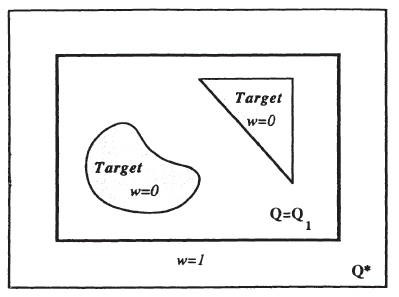
\includegraphics[scale=1]{bvpregions}
\caption{A state space divided into capture,escape, and regions of play \cite{bardi2}}
\label{bvpregions}
\end{figure}
\clearpage
\newpage

\begin{figure}
\vspace{2.4in}
\centering
\begin{subfigure}[b]{0.475\textwidth}
	\centering
	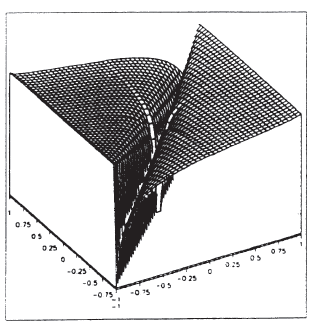
\includegraphics[width=\textwidth]{bvpresult1}
	\caption{Approximate value function when $v_1 = 1$, $v_2 = 1$}
	\label{bvpresult1}
\end{subfigure}
\hfill
\begin{subfigure}[b]{0.475\textwidth}
	\centering
	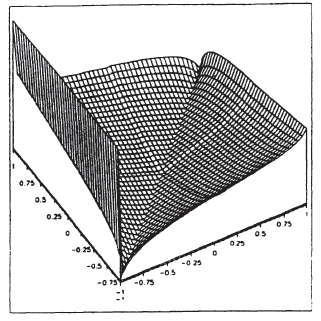
\includegraphics[width=\textwidth]{bvpresult2}
	\caption{Approximate value function when $v_1 = 5$, $v_2 = 1$}
	\label{bvpresult2}
\end{subfigure}
\caption{Results for one-dimensional pursuit-evasion games \cite{bardi2}}
\label{bvpresults}
\end{figure}
\clearpage
\newpage

\begin{figure}
\vspace{2.4in}
\centering
\begin{subfigure}[b]{0.475\textwidth}
	\centering
	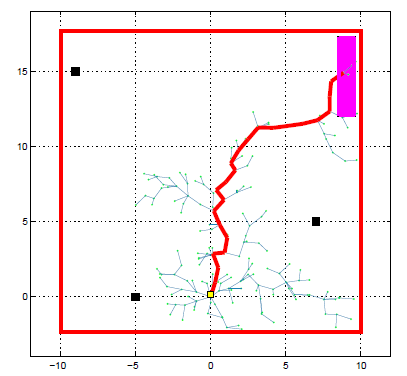
\includegraphics[width=\textwidth]{rrt500}
	\caption{Pursuit-Evasion $\textnormal{RRT}^*$ run for 500 iterations }
	\label{rrt500}
\end{subfigure}
\hfill
\begin{subfigure}[b]{0.475\textwidth}
	\centering
	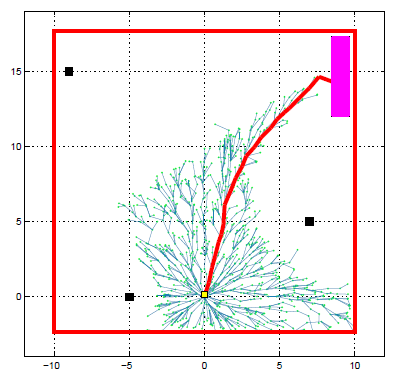
\includegraphics[width=\textwidth]{rrt3000}
	\caption{Pursuit-Evasion $\textnormal{RRT}^*$ run for 3000 iterations}
	\label{rrt3000}
\end{subfigure}
\vskip\baselineskip
\begin{subfigure}[b]{0.475\textwidth}
	\centering
	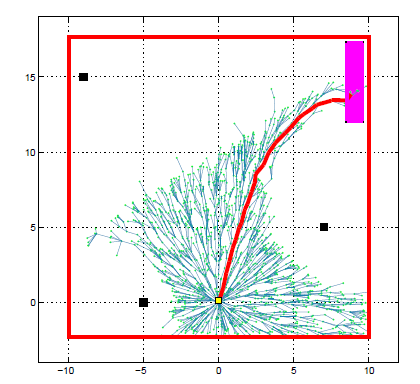
\includegraphics[width=\textwidth]{rrt5000}
	\caption{Pursuit-Evasion $\textnormal{RRT}^*$ run for 5000 iterations}
	\label{rrt5000}
\end{subfigure}
\quad
\begin{subfigure}[b]{0.475\textwidth}
	\centering
	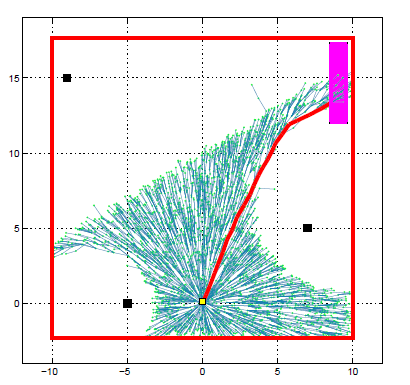
\includegraphics[width=\textwidth]{rrt10000}
	\caption{Pursuit-Evasion $\textnormal{RRT}^*$ run for 10000 iterations}
	\label{rrt10000}
\end{subfigure}
\caption{Pursuit-Evasion $\textnormal{RRT}^*$ \cite{karaman}}
\label{rrtfig}
\end{figure}
\clearpage
\newpage

\begin{figure}
\vspace{2.4in}
\centering
\begin{subfigure}[b]{0.475\textwidth}
	\centering
	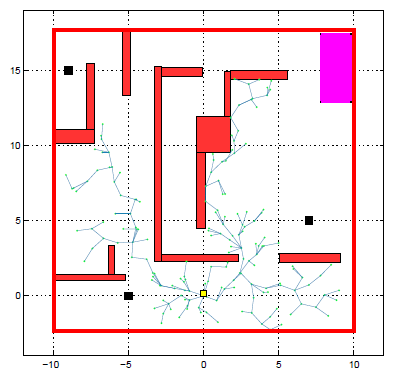
\includegraphics[width=\textwidth]{rrtobs500}
	\caption{Pursuit-Evasion $\textnormal{RRT}^*$ run for 500 iterations}
	\label{rrtobs500}
\end{subfigure}
\hfill
\begin{subfigure}[b]{0.475\textwidth}
	\centering
	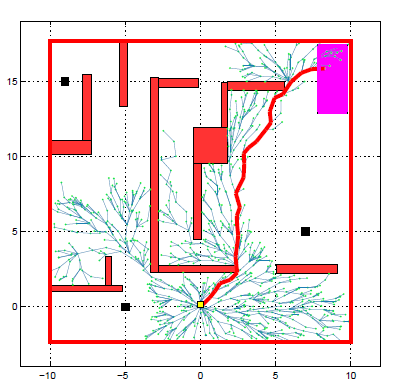
\includegraphics[width=\textwidth]{rrtobs3000}
	\caption{Pursuit-Evasion $\textnormal{RRT}^*$ run for 3000 iterations}
	\label{rrtobs3000}
\end{subfigure}
\vskip\baselineskip
\begin{subfigure}[b]{0.475\textwidth}
	\centering
	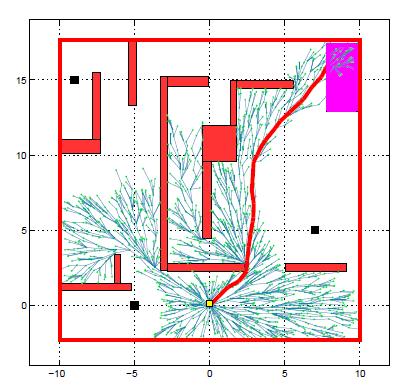
\includegraphics[width=\textwidth]{rrtobs5000}
	\caption{Pursuit-Evasion $\textnormal{RRT}^*$ run for 5000 iterations}
	\label{rrtobs5000}
\end{subfigure}
\quad
\begin{subfigure}[b]{0.475\textwidth}
	\centering
	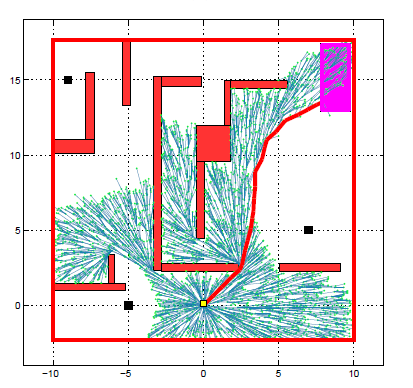
\includegraphics[width=\textwidth]{rrtobs10000}
	\caption{Pursuit-Evasion $\textnormal{RRT}^*$ run for 10000 iterations}
	\label{rrtobs10000}
\end{subfigure}
\caption{Pursuit-Evasion $\textnormal{RRT}^*$ in a field with obstacles\cite{karaman}}
\label{rrtobsfig}
\end{figure}
\clearpage
\newpage

\begin{figure}
\vspace{2.4in}
\centering
\begin{subfigure}[b]{0.475\textwidth}
	\centering
	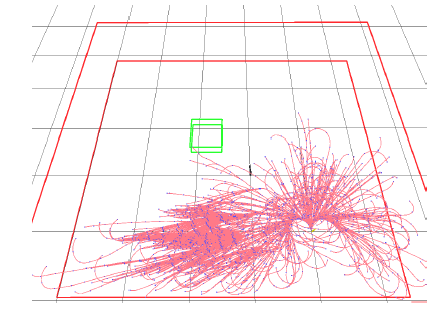
\includegraphics[width=\textwidth]{rrtdubins}
	\caption{Pursuit-Evasion $\textnormal{RRT}^*$ run for 3000 iterations}
	\label{rrtdubins}
\end{subfigure}
\hfill
\begin{subfigure}[b]{0.475\textwidth}
	\centering
	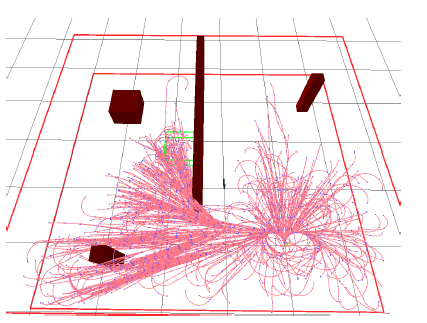
\includegraphics[width=\textwidth]{rrtobsdubins}
	\caption{Pursuit-Evasion $\textnormal{RRT}^*$ run for 3000 iterations in a field with obstacles}
	\label{rrtobsdubins}
\end{subfigure}
\caption{Pursuit-Evasion $\textnormal{RRT}^*$ on a problem with Dubins dynamics \cite{karaman}}
\label{rrtdubinsfig}
\end{figure}
\clearpage
\newpage

\begin{figure}
\vspace{2.4in}
\centering
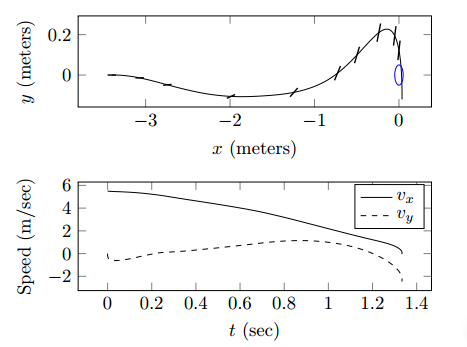
\includegraphics[scale=1]{gorodglide}
\caption{Optimal glide path with vertical and horizontal velocities \cite{gorod}}
\label{gorodglide}
\end{figure}
\clearpage
\newpage

\begin{figure}
\vspace{2.4in}
\centering
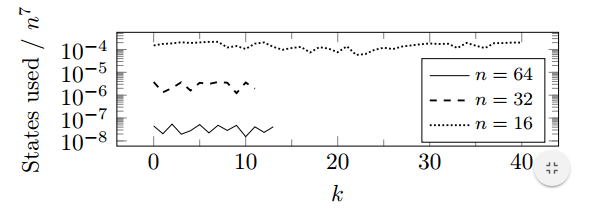
\includegraphics[scale=1]{gorodstates}
\caption{Fraction of states evaluated by TTVI in optimal glide problem \cite{gorod}}
\label{gorodstates}
\end{figure}
\clearpage
\newpage

\begin{figure}
\vspace{2.4in}
\centering
\includegraphics[scale=3]{VIpursplot1}
\caption{Pursuer at (1,1) captures stationary evader at (5,5) after the first Pursuit Value Iteration Run}
\label{VIpursplot1}
\end{figure}
\clearpage
\newpage

\begin{figure}
\vspace{2.4in}
\centering
\includegraphics[scale=3]{VIpursplot2}
\caption{Pursuer at (5,1) captures stationary evader at (5,5) after the first Pursuit Value Iteration Run}
\label{VIpursplot2}
\end{figure}
\clearpage
\newpage

\begin{figure}
\vspace{2.4in}
\centering
\includegraphics[scale=3]{VIpursplot3}
\caption{Pursuer at (9,1) captures stationary evader at (5,5) after the first Pursuit Value Iteration Run}
\label{VIpursplot3}
\end{figure}
\clearpage
\newpage

\begin{figure}
\vspace{2.4in}
\centering
\includegraphics[scale=3]{VIpursplot4}
\caption{Pursuer at (9,5) captures stationary evader at (5,5) after the first Pursuit Value Iteration Run}
\label{VIpursplot4}
\end{figure}
\clearpage
\newpage

\begin{figure}
\vspace{2.4in}
\centering
\includegraphics[scale=3]{VIpursplot5}
\caption{Pursuer at (9,9) captures stationary evader at (5,5) after the first Pursuit Value Iteration Run}
\label{VIpursplot5}
\end{figure}
\clearpage
\newpage

\begin{figure}
\vspace{2.4in}
\centering
\includegraphics[scale=3]{VIpursplot6}
\caption{Pursuer at (5,9) captures stationary evader at (5,5) after the first Pursuit Value Iteration Run}
\label{VIpursplot6}
\end{figure}
\clearpage
\newpage

\begin{figure}
\vspace{2.4in}
\centering
\includegraphics[scale=3]{VIpursplot7}
\caption{Pursuer at (1,9) captures stationary evader at (5,5) after the first Pursuit Value Iteration Run}
\label{VIpursplot7}
\end{figure}
\clearpage
\newpage

\begin{figure}
\vspace{2.4in}
\centering
\includegraphics[scale=3]{VIpursplot8}
\caption{Pursuer at (1,5) captures stationary evader at (5,5) after the first Pursuit Value Iteration Run}
\label{VIpursplot8}
\end{figure}
\clearpage
\newpage

\begin{figure}
\vspace{2.4in}
\centering
\includegraphics[scale=0.25]{VIpursue0}
\caption{State Cost of the Pursuer when the Evader is at (5,5) after one iteration}
\label{VIpursue0}
\end{figure}
\clearpage
\newpage

\begin{figure}
\vspace{2.4in}
\centering
\includegraphics[scale=0.25]{VIpursue10}
\caption{State Cost of the Pursuer when the Evader is at (5,5) after eleven iterations}
\label{VIpursue10}
\end{figure}
\clearpage
\newpage

\begin{figure}
\vspace{2.4in}
\centering
\includegraphics[scale=0.25]{VIpursue98}
\caption{State Cost of the Pursuer when the Evader is at (5,5) after ninety-nine iterations}
\label{VIpursue98}
\end{figure}
\clearpage
\newpage

\begin{figure}
\vspace{2.4in}
\centering
\includegraphics[scale=0.25]{VIpursue99}
\caption{State Cost of the Pursuer when the Evader is at (5,5) after a hundred iterations}
\label{VIpursue99}
\end{figure}
\clearpage
\newpage

\begin{figure}
\vspace{2.4in}
\centering
\includegraphics[scale=3]{VIevadplot1}
\caption{Evader at (5,5) evades stationary pursuer at (1,1) after the first Evade Value Iteration Run}
\label{VIevadplot1}
\end{figure}
\clearpage
\newpage

\begin{figure}
\vspace{2.4in}
\centering
\includegraphics[scale=3]{VIevadplot2}
\caption{Evader at (5,5) evades stationary pursuer at (5,1) after the first Evade Value Iteration Run}
\label{VIevadplot2}
\end{figure}
\clearpage
\newpage

\begin{figure}
\vspace{2.4in}
\centering
\includegraphics[scale=3]{VIevadplot3}
\caption{Evader at (5,5) evades stationary pursuer at (9,1) after the first Evade Value Iteration Run}
\label{VIevadplot3}
\end{figure}
\clearpage
\newpage

\begin{figure}
\vspace{2.4in}
\centering
\includegraphics[scale=3]{VIevadplot4}
\caption{Evader at (5,5) evades stationary pursuer at (9,5) after the first Evade Value Iteration Run}
\label{VIevadplot4}
\end{figure}
\clearpage
\newpage

\begin{figure}
\vspace{2.4in}
\centering
\includegraphics[scale=3]{VIevadplot5}
\caption{Evader at (5,5) evades stationary pursuer at (9,9) after the first Evade Value Iteration Run}
\label{VIevadplot5}
\end{figure}
\clearpage
\newpage

\begin{figure}
\vspace{2.4in}
\centering
\includegraphics[scale=3]{VIevadplot6}
\caption{Evader at (5,5) evades stationary pursuer at (5,9) after the first Evade Value Iteration Run}
\label{VIevadplot6}
\end{figure}
\clearpage
\newpage

\begin{figure}
\vspace{2.4in}
\centering
\includegraphics[scale=3]{VIevadplot7}
\caption{Evader at (5,5) evades stationary pursuer at (1,9) after the first Evade Value Iteration Run}
\label{VIevadplot7}
\end{figure}
\clearpage
\newpage

\begin{figure}
\vspace{2.4in}
\centering
\includegraphics[scale=3]{VIevadplot8}
\caption{Evader at (5,5) evades stationary pursuer at (1,5) after the first Evade Value Iteration Run}
\label{VIevadplot8}
\end{figure}
\clearpage
\newpage

\begin{figure}
\vspace{2.4in}
\centering
\includegraphics[scale=0.25]{VIevade0}
\caption{State Cost of the Evader when the Pursuer is at (1,1) after one iteration}
\label{VIevade0}
\end{figure}
\clearpage
\newpage

\begin{figure}
\vspace{2.4in}
\centering
\includegraphics[scale=0.25]{VIevade10}
\caption{State Cost of the Evader when the Pursuer is at (1,1) after elven iterations}
\label{VIevade10}
\end{figure}
\clearpage
\newpage

\begin{figure}
\vspace{2.4in}
\centering
\includegraphics[scale=0.25]{VIevade98}
\caption{State Cost of the Evader when the Pursuer is at (1,1) after ninety-nine iterations}
\label{VIevade98}
\end{figure}
\clearpage
\newpage

\begin{figure}
\vspace{2.4in}
\centering
\includegraphics[scale=0.25]{VIevade99}
\caption{State Cost of the Evader when the Pursuer is at (1,1) after a hundred iterations}
\label{VIevade99}
\end{figure}
\clearpage
\newpage

\begin{figure}
\vspace{2.4in}
\centering
\includegraphics[scale=3]{VIpursbr1plot1}
\caption{Pursuer at (1,1) captures evader at (5,5) after the second Pursuit Value Iteration Run}
\label{VIpursbr1plot1}
\end{figure}
\clearpage
\newpage

\begin{figure}
\vspace{2.4in}
\centering
\includegraphics[scale=3]{VIpursbr1plot2}
\caption{Pursuer at (5,1) captures evader at (5,5) after the second Pursuit Value Iteration Run}
\label{VIpursbr1plot2}
\end{figure}
\clearpage
\newpage

\begin{figure}
\vspace{2.4in}
\centering
\includegraphics[scale=3]{VIpursbr1plot3}
\caption{Pursuer at (9,1) captures evader at (5,5) after the second Pursuit Value Iteration Run}
\label{VIpursbr1plot3}
\end{figure}
\clearpage
\newpage

\begin{figure}
\vspace{2.4in}
\centering
\includegraphics[scale=3]{VIpursbr1plot4}
\caption{Pursuer at (9,5) captures evader at (5,5) after the second Pursuit Value Iteration Run}
\label{VIpursbr1plot4}
\end{figure}
\clearpage
\newpage

\begin{figure}
\vspace{2.4in}
\centering
\includegraphics[scale=3]{VIpursbr1plot5}
\caption{Pursuer at (9,9) captures evader at (5,5) after the second Pursuit Value Iteration Run}
\label{VIpursbr1plot5}
\end{figure}
\clearpage
\newpage

\begin{figure}
\vspace{2.4in}
\centering
\includegraphics[scale=3]{VIpursbr1plot6}
\caption{Pursuer at (5,9) captures evader at (5,5) after the second Pursuit Value Iteration Run}
\label{VIpursbr1plot6}
\end{figure}
\clearpage
\newpage

\begin{figure}
\vspace{2.4in}
\centering
\includegraphics[scale=3]{VIpursbr1plot7}
\caption{Pursuer at (1,9) captures evader at (5,5) after the second Pursuit Value Iteration Run}
\label{VIpursbr1plot7}
\end{figure}
\clearpage
\newpage

\begin{figure}
\vspace{2.4in}
\centering
\includegraphics[scale=3]{VIpursbr1plot8}
\caption{Pursuer at (1,5) captures evader at (5,5) after the second Pursuit Value Iteration Run}
\label{VIpursbr1plot8}
\end{figure}
\clearpage
\newpage

\begin{figure}
\vspace{2.4in}
\centering
\includegraphics[scale=0.25]{VIpursue1br0}
\caption{State Cost of the Pursuer when the Evader is at (5,5) after one iteration}
\label{VIpursue1br0}
\end{figure}
\clearpage
\newpage

\begin{figure}
\vspace{2.4in}
\centering
\includegraphics[scale=0.25]{VIpursue1br10}
\caption{State Cost of the Pursuer when the Evader is at (5,5) after eleven iterations}
\label{VIpursue1br10}
\end{figure}
\clearpage
\newpage

\begin{figure}
\vspace{2.4in}
\centering
\includegraphics[scale=0.25]{VIpursue1br98}
\caption{State Cost of the Pursuer when the Evader is at (5,5) after ninety-nine iterations}
\label{VIpursue1br98}
\end{figure}
\clearpage
\newpage

\begin{figure}
\vspace{2.4in}
\centering
\includegraphics[scale=0.25]{VIpursue1br99}
\caption{State Cost of the Pursuer when the Evader is at (5,5) after a hundred iterations}
\label{VIpursue1br99}
\end{figure}
\clearpage
\newpage

\begin{figure}
\vspace{2.4in}
\centering
\includegraphics[scale=3]{VIevadbrplot1}
\caption{Pursuer at (1,1) captures evader at (5,5) after the second Evade Value Iteration Run}
\label{VIevadbrplot1}
\end{figure}
\clearpage
\newpage

\begin{figure}
\vspace{2.4in}
\centering
\includegraphics[scale=3]{VIevadbrplot2}
\caption{Pursuer at (5,1) captures evader at (5,5) after the second Evade Value Iteration Run}
\label{VIevadbrplot2}
\end{figure}
\clearpage
\newpage

\begin{figure}
\vspace{2.4in}
\centering
\includegraphics[scale=3]{VIevadbrplot3}
\caption{Pursuer at (9,1) captures evader at (5,5) after the second Evade Value Iteration Run}
\label{VIevadbrplot3}
\end{figure}
\clearpage
\newpage

\begin{figure}
\vspace{2.4in}
\centering
\includegraphics[scale=3]{VIevadbrplot4}
\caption{Pursuer at (9,5) captures evader at (5,5) after the second Evade Value Iteration Run}
\label{VIevadbrplot4}
\end{figure}
\clearpage
\newpage

\begin{figure}
\vspace{2.4in}
\centering
\includegraphics[scale=3]{VIevadbrplot5}
\caption{Pursuer at (9,9) captures evader at (5,5) after the second Evade Value Iteration Run}
\label{VIevadbrplot5}
\end{figure}
\clearpage
\newpage

\begin{figure}
\vspace{2.4in}
\centering
\includegraphics[scale=3]{VIevadbrplot6}
\caption{Pursuer at (5,9) captures evader at (5,5) after the second Evade Value Iteration Run}
\label{VIevadbrplot6}
\end{figure}
\clearpage
\newpage

\begin{figure}
\vspace{2.4in}
\centering
\includegraphics[scale=3]{VIevadbrplot7}
\caption{Pursuer at (1,9) captures evader at (5,5) after the second Evade Value Iteration Run}
\label{VIevadbrplot7}
\end{figure}
\clearpage
\newpage

\begin{figure}
\vspace{2.4in}
\centering
\includegraphics[scale=3]{VIevadbrplot8}
\caption{Pursuer at (1,5) captures evader at (5,5) after the second Evade Value Iteration Run}
\label{VIevadbrplot8}
\end{figure}
\clearpage
\newpage

\begin{figure}
\vspace{2.4in}
\centering
\includegraphics[scale=0.25]{VIevadebr0}
\caption{State Cost of the Evader when the Pursuer is at (1,1) after one iteration}
\label{VIevadebr0}
\end{figure}
\clearpage
\newpage

\begin{figure}
\vspace{2.4in}
\centering
\includegraphics[scale=0.25]{VIevadebr10}
\caption{State Cost of the Evader when the Pursuer is at (1,1) after elven iterations}
\label{VIevadebr10}
\end{figure}
\clearpage
\newpage

\begin{figure}
\vspace{2.4in}
\centering
\includegraphics[scale=0.25]{VIevadebr98}
\caption{State Cost of the Evader when the Pursuer is at (1,1) after ninety-nine iterations}
\label{VIevadebr98}
\end{figure}
\clearpage
\newpage

\begin{figure}
\vspace{2.4in}
\centering
\includegraphics[scale=0.25]{VIevadebr99}
\caption{State Cost of the Evader when the Pursuer is at (1,1) after a hundred iterations}
\label{VIevadebr99}
\end{figure}
\clearpage
\newpage

\begin{figure}
\vspace{2.4in}
\centering
\includegraphics[scale=3]{VIpursbr2plot1}
\caption{Pursuer at (1,1) captures evader at (5,5) after the third Pursuit Value Iteration Run}
\label{VIpursbr2plot1}
\end{figure}
\clearpage
\newpage

\begin{figure}
\vspace{2.4in}
\centering
\includegraphics[scale=3]{VIpursbr2plot2}
\caption{Pursuer at (5,1) captures evader at (5,5) after the third Pursuit Value Iteration Run}
\label{VIpursbr2plot2}
\end{figure}
\clearpage
\newpage

\begin{figure}
\vspace{2.4in}
\centering
\includegraphics[scale=3]{VIpursbr2plot3}
\caption{Pursuer at (9,1) captures evader at (5,5) after the third Pursuit Value Iteration Run}
\label{VIpursbr2plot3}
\end{figure}
\clearpage
\newpage

\begin{figure}
\vspace{2.4in}
\centering
\includegraphics[scale=3]{VIpursbr2plot4}
\caption{Pursuer at (9,5) captures evader at (5,5) after the third Pursuit Value Iteration Run}
\label{VIpursbr2plot4}
\end{figure}
\clearpage
\newpage

\begin{figure}
\vspace{2.4in}
\centering
\includegraphics[scale=3]{VIpursbr2plot5}
\caption{Pursuer at (9,9) captures evader at (5,5) after the third Pursuit Value Iteration Run}
\label{VIpursbr2plot5}
\end{figure}
\clearpage
\newpage

\begin{figure}
\vspace{2.4in}
\centering
\includegraphics[scale=3]{VIpursbr2plot6}
\caption{Pursuer at (5,9) captures evader at (5,5) after the third Pursuit Value Iteration Run}
\label{VIpursbr2plot6}
\end{figure}
\clearpage
\newpage

\begin{figure}
\vspace{2.4in}
\centering
\includegraphics[scale=3]{VIpursbr2plot7}
\caption{Pursuer at (1,9) captures evader at (5,5) after the third Pursuit Value Iteration Run}
\label{VIpursbr2plot7}
\end{figure}
\clearpage
\newpage

\begin{figure}
\vspace{2.4in}
\centering
\includegraphics[scale=3]{VIpursbr2plot8}
\caption{Pursuer at (1,5) captures evader at (5,5) after the third Pursuit Value Iteration Run}
\label{VIpursbr2plot8}
\end{figure}
\clearpage
\newpage

\begin{figure}
\vspace{2.4in}
\centering
\includegraphics[scale=0.25]{VIpursue2br0}
\caption{State Cost of the Pursuer when the Evader is at (5,5) after one iteration}
\label{VIpursue2br0}
\end{figure}
\clearpage
\newpage

\begin{figure}
\vspace{2.4in}
\centering
\includegraphics[scale=0.25]{VIpursue2br99}
\caption{State Cost of the Pursuer when the Evader is at (5,5) after a hundred iterations}
\label{VIpursue2br99}
\end{figure}
\clearpage
\newpage

\begin{figure}
\vspace{2.4in}
\centering
\includegraphics[scale=3]{4DTradPurs0diffNormplot}
\caption{Change in Norm of Pursuer State Value for each iteration of traditional VI}
\label{4DTradPurs0diffNormplot}
\end{figure}
\clearpage
\newpage

\begin{figure}
\vspace{2.4in}
\centering
\includegraphics[scale=3]{4DTradPurs0normplot}
\caption{Norm of Pursuer State Value for each iteration of traditional VI}
\label{4DTradPurs0normplot}
\end{figure}
\clearpage
\newpage

\begin{figure}
\vspace{2.4in}
\centering
\includegraphics[scale=3]{4DTradEvad0diffNormplot}
\caption{Change in Norm of Evader State Value for each iteration of traditional VI}
\label{4DTradEvad0diffNormplot}
\end{figure}
\clearpage
\newpage

\begin{figure}
\vspace{2.4in}
\centering
\includegraphics[scale=3]{4DTradEvad0normplot}
\caption{Norm of Evader State Value for each iteration of traditional VI}
\label{4DTradEvad0normplot}
\end{figure}
\clearpage
\newpage

\begin{figure}
\vspace{2.4in}
\centering
\includegraphics[scale=3]{4DTradPurs1diffNormplot}
\caption{Change in Norm of Pursuer State Value for each iteration of traditional VI}
\label{4DTradPurs1diffNormplot}
\end{figure}
\clearpage
\newpage

\begin{figure}
\vspace{2.4in}
\centering
\includegraphics[scale=3]{4DTradPurs1normplot}
\caption{Norm of Pursuer State Value for each iteration of traditional VI}
\label{4DTradPurs1normplot}
\end{figure}
\clearpage
\newpage

\begin{figure}
\vspace{2.4in}
\centering
\includegraphics[scale=3]{4DTradPurspurscolorplot}
\caption{Pursuer State Value when Evader is at (5,5)}
\label{4DTradPurspurscolorplot}
\end{figure}
\clearpage
\newpage

\begin{figure}
\vspace{2.4in}
\centering
\includegraphics[scale=3]{4DTradEvad1diffNormplot}
\caption{Change in Norm of Evader State Value for each iteration of traditional VI}
\label{4DTradEvad1diffNormplot}
\end{figure}
\clearpage
\newpage

\begin{figure}
\vspace{2.4in}
\centering
\includegraphics[scale=3]{4DTradEvad1normplot}
\caption{Norm of Evader State Value for each iteration of traditional VI}
\label{4DTradEvad1normplot}
\end{figure}
\clearpage
\newpage

\begin{figure}
\vspace{2.4in}
\centering
\includegraphics[scale=3]{4DTradEvadevadcolorplot}
\caption{Evader State Value when Pursuer is at (1,1)}
\label{4DTradEvadevadcolorplot}
\end{figure}
\clearpage
\newpage

\begin{figure}
\vspace{2.4in}
\centering
\includegraphics[scale=3]{4DTradEvadmovieplot0}
\caption{Start of pursuit-Evasion game with pursuer starting at (1,1) and the evader starting at (5,5)}
\label{4DTradEvadmovieplot0}
\end{figure}
\clearpage
\newpage

\begin{figure}
\vspace{2.4in}
\centering
\includegraphics[scale=3]{4DTradEvadmovieplot1}
\caption{Pursuit-Evasion game with pursuer starting at (1,1) and the evader starting at (5,5) after 1 second}
\label{4DTradEvadmovieplot1}
\end{figure}
\clearpage
\newpage

\begin{figure}
\vspace{2.4in}
\centering
\includegraphics[scale=3]{4DTradEvadmovieplot2}
\caption{Pursuit-Evasion game with pursuer starting at (1,1) and the evader starting at (5,5) after 2 second}
\label{4DTradEvadmovieplot2}
\end{figure}
\clearpage
\newpage

\begin{figure}
\vspace{2.4in}
\centering
\includegraphics[scale=3]{4DTradEvadmovieplot3}
\caption{Pursuit-Evasion game with pursuer starting at (1,1) and the evader starting at (5,5) after 3 second}
\label{4DTradEvadmovieplot3}
\end{figure}
\clearpage
\newpage

\begin{figure}
\vspace{2.4in}
\centering
\includegraphics[scale=3]{4DTradEvadmovieplot4}
\caption{Pursuit-Evasion game with pursuer starting at (1,1) and the evader starting at (5,5) after 4 second}
\label{4DTradEvadmovieplot4}
\end{figure}
\clearpage
\newpage

\begin{figure}
\vspace{2.4in}
\centering
\includegraphics[scale=3]{4DTradEvadmovieplot5}
\caption{Pursuit-Evasion game with pursuer starting at (1,1) and the evader starting at (5,5) after 5 second}
\label{4DTradEvadmovieplot5}
\end{figure}
\clearpage
\newpage

\begin{figure}
\vspace{2.4in}
\centering
\includegraphics[scale=3]{4DTradEvadmovieplot6}
\caption{Pursuit-Evasion game with pursuer starting at (1,1) and the evader starting at (5,5) after 6 second}
\label{4DTradEvadmovieplot6}
\end{figure}
\clearpage
\newpage

\begin{figure}
\vspace{2.4in}
\centering
\includegraphics[scale=3]{4DTradEvadmovieplot7}
\caption{Pursuit-Evasion game with pursuer starting at (1,1) and the evader starting at (5,5) after 7 second}
\label{4DTradEvadmovieplot7}
\end{figure}
\clearpage
\newpage

\begin{figure}
\vspace{2.4in}
\centering
\includegraphics[scale=3]{4DTradEvadmovieplot8}
\caption{Pursuit-Evasion game with pursuer starting at (1,1) and the evader starting at (5,5) after 8 second}
\label{4DTradEvadmovieplot8}
\end{figure}
\clearpage
\newpage

\begin{figure}
\vspace{2.4in}
\centering
\includegraphics[scale=3]{4DTradEvadmovieplot9}
\caption{Pursuit-Evasion game with pursuer starting at (1,1) and the evader starting at (5,5) after 9 second}
\label{4DTradEvadmovieplot9}
\end{figure}
\clearpage
\newpage

\begin{figure}
\vspace{2.4in}
\centering
\includegraphics[scale=3]{4DTradEvadphaseplot}
\caption{Pursuit-Evasion game with pursuer starting at (1,1) and the evader starting at (5,5) at one second intervals}
\label{4DTradEvadphaseplot}
\end{figure}
\clearpage
\newpage

\begin{figure}
\vspace{2.4in}
\centering
\includegraphics[scale=3]{4DTradEvadrelplot}
\caption{Relative position between pursuer starting at (1,1) and the evader starting at (5,5)}
\label{4DTradEvadrelplot}
\end{figure}
\clearpage
\newpage

\begin{figure}
\vspace{2.4in}
\centering
\includegraphics[scale=3]{4DCompPurs0diffNormplot}
\caption{Change in Norm of Pursuer State Value for each iteration of traditional VI}
\label{4DCompPurs0diffNormplot}
\end{figure}
\clearpage
\newpage

\begin{figure}
\vspace{2.4in}
\centering
\includegraphics[scale=3]{4DCompPurs0normplot}
\caption{Norm of Pursuer State Value for each iteration of traditional VI}
\label{4DCompPurs0normplot}
\end{figure}
\clearpage
\newpage

\begin{figure}
\vspace{2.4in}
\centering
\includegraphics[scale=3]{4DCompEvad0diffNormplot}
\caption{Change in Norm of Evader State Value for each iteration of traditional VI}
\label{4DCompEvad0diffNormplot}
\end{figure}
\clearpage
\newpage

\begin{figure}
\vspace{2.4in}
\centering
\includegraphics[scale=3]{4DCompEvad0normplot}
\caption{Norm of Evader State Value for each iteration of traditional VI}
\label{4DCompEvad0normplot}
\end{figure}
\clearpage
\newpage

\begin{figure}
\vspace{2.4in}
\centering
\includegraphics[scale=3]{4DCompPurs1diffNormplot}
\caption{Change in Norm of Pursuer State Value for each iteration of traditional VI}
\label{4DCompPurs1diffNormplot}
\end{figure}
\clearpage
\newpage

\begin{figure}
\vspace{2.4in}
\centering
\includegraphics[scale=3]{4DCompPurs1normplot}
\caption{Norm of Pursuer State Value for each iteration of traditional VI}
\label{4DCompPurs1normplot}
\end{figure}
\clearpage
\newpage

\begin{figure}
\vspace{2.4in}
\centering
\includegraphics[scale=3]{4DCompPurspurscolorplot}
\caption{Pursuer State Value when Evader is at (5,5)}
\label{4DCompPurspurscolorplot}
\end{figure}
\clearpage
\newpage

\begin{figure}
\vspace{2.4in}
\centering
\includegraphics[scale=3]{4DCompEvad1diffNormplot}
\caption{Change in Norm of Evader State Value for each iteration of traditional VI}
\label{4DCompEvad1diffNormplot}
\end{figure}
\clearpage
\newpage

\begin{figure}
\vspace{2.4in}
\centering
\includegraphics[scale=3]{4DCompEvad1normplot}
\caption{Norm of Evader State Value for each iteration of traditional VI}
\label{4DCompEvad1normplot}
\end{figure}
\clearpage
\newpage

\begin{figure}
\vspace{2.4in}
\centering
\includegraphics[scale=3]{4DCompEvadevadcolorplot}
\caption{Evader State Value when Pursuer is at (1,1)}
\label{4DCompEvadevadcolorplot}
\end{figure}
\clearpage
\newpage

\begin{figure}
\vspace{2.4in}
\centering
\includegraphics[scale=3]{4DCompEvadmovieplot0}
\caption{Start of pursuit-Evasion game with pursuer starting at (1,1) and the evader starting at (5,5)}
\label{4DCompEvadmovieplot0}
\end{figure}
\clearpage
\newpage

\begin{figure}
\vspace{2.4in}
\centering
\includegraphics[scale=3]{4DCompEvadmovieplot1}
\caption{Pursuit-Evasion game with pursuer starting at (1,1) and the evader starting at (5,5) after 1 second}
\label{4DCompEvadmovieplot1}
\end{figure}
\clearpage
\newpage

\begin{figure}
\vspace{2.4in}
\centering
\includegraphics[scale=3]{4DCompEvadmovieplot2}
\caption{Pursuit-Evasion game with pursuer starting at (1,1) and the evader starting at (5,5) after 2 second}
\label{4DCompEvadmovieplot2}
\end{figure}
\clearpage
\newpage

\begin{figure}
\vspace{2.4in}
\centering
\includegraphics[scale=3]{4DCompEvadmovieplot3}
\caption{Pursuit-Evasion game with pursuer starting at (1,1) and the evader starting at (5,5) after 3 second}
\label{4DCompEvadmovieplot3}
\end{figure}
\clearpage
\newpage

\begin{figure}
\vspace{2.4in}
\centering
\includegraphics[scale=3]{4DCompEvadmovieplot4}
\caption{Pursuit-Evasion game with pursuer starting at (1,1) and the evader starting at (5,5) after 4 second}
\label{4DCompEvadmovieplot4}
\end{figure}
\clearpage
\newpage

\begin{figure}
\vspace{2.4in}
\centering
\includegraphics[scale=3]{4DCompEvadmovieplot5}
\caption{Pursuit-Evasion game with pursuer starting at (1,1) and the evader starting at (5,5) after 5 second}
\label{4DCompEvadmovieplot5}
\end{figure}
\clearpage
\newpage

\begin{figure}
\vspace{2.4in}
\centering
\includegraphics[scale=3]{4DCompEvadmovieplot6}
\caption{Pursuit-Evasion game with pursuer starting at (1,1) and the evader starting at (5,5) after 6 second}
\label{4DCompEvadmovieplot6}
\end{figure}
\clearpage
\newpage

\begin{figure}
\vspace{2.4in}
\centering
\includegraphics[scale=3]{4DCompEvadmovieplot7}
\caption{Pursuit-Evasion game with pursuer starting at (1,1) and the evader starting at (5,5) after 7 second}
\label{4DCompEvadmovieplot7}
\end{figure}
\clearpage
\newpage

\begin{figure}
\vspace{2.4in}
\centering
\includegraphics[scale=3]{4DCompEvadmovieplot8}
\caption{Pursuit-Evasion game with pursuer starting at (1,1) and the evader starting at (5,5) after 8 second}
\label{4DCompEvadmovieplot8}
\end{figure}
\clearpage
\newpage

\begin{figure}
\vspace{2.4in}
\centering
\includegraphics[scale=3]{4DCompEvadmovieplot9}
\caption{Pursuit-Evasion game with pursuer starting at (1,1) and the evader starting at (5,5) after 9 second}
\label{4DCompEvadmovieplot9}
\end{figure}
\clearpage
\newpage

\begin{figure}
\vspace{2.4in}
\centering
\includegraphics[scale=3]{4DCompEvadphaseplot}
\caption{Pursuit-Evasion game with pursuer starting at (1,1) and the evader starting at (5,5) at one second intervals}
\label{4DCompEvadphaseplot}
\end{figure}
\clearpage
\newpage

\begin{figure}
\vspace{2.4in}
\centering
\includegraphics[scale=3]{4DCompEvadrelplot}
\caption{Relative position between pursuer starting at (1,1) and the evader starting at (5,5)}
\label{4DCompEvadrelplot}
\end{figure}
\clearpage
\newpage

\begin{figure}
\vspace{2.4in}
\centering
\includegraphics[scale=3]{TTVIpursplot1}
\caption{Pursuer at (1,1) captures stationary evader at (5,5) after the first Pursuit Value Iteration Run}
\label{TTVIpursplot1}
\end{figure}
\clearpage
\newpage

\begin{figure}
\vspace{2.4in}
\centering
\includegraphics[scale=3]{TTVIpursplot2}
\caption{Pursuer at (5,1) captures stationary evader at (5,5) after the first Pursuit Value Iteration Run}
\label{TTVIpursplot2}
\end{figure}
\clearpage
\newpage

\begin{figure}
\vspace{2.4in}
\centering
\includegraphics[scale=3]{TTVIpursplot3}
\caption{Pursuer at (9,1) captures stationary evader at (5,5) after the first Pursuit Value Iteration Run}
\label{TTVIpursplot3}
\end{figure}
\clearpage
\newpage

\begin{figure}
\vspace{2.4in}
\centering
\includegraphics[scale=3]{TTVIpursplot4}
\caption{Pursuer at (9,5) captures stationary evader at (5,5) after the first Pursuit Value Iteration Run}
\label{TTVIpursplot4}
\end{figure}
\clearpage
\newpage

\begin{figure}
\vspace{2.4in}
\centering
\includegraphics[scale=3]{TTVIpursplot5}
\caption{Pursuer at (9,9) captures stationary evader at (5,5) after the first Pursuit Value Iteration Run}
\label{TTVIpursplot5}
\end{figure}
\clearpage
\newpage

\begin{figure}
\vspace{2.4in}
\centering
\includegraphics[scale=3]{TTVIpursplot6}
\caption{Pursuer at (5,9) captures stationary evader at (5,5) after the first Pursuit Value Iteration Run}
\label{TTVIpursplot6}
\end{figure}
\clearpage
\newpage

\begin{figure}
\vspace{2.4in}
\centering
\includegraphics[scale=3]{TTVIpursplot7}
\caption{Pursuer at (1,9) captures stationary evader at (5,5) after the first Pursuit Value Iteration Run}
\label{TTVIpursplot7}
\end{figure}
\clearpage
\newpage

\begin{figure}
\vspace{2.4in}
\centering
\includegraphics[scale=3]{TTVIpursplot8}
\caption{Pursuer at (1,5) captures stationary evader at (5,5) after the first Pursuit Value Iteration Run}
\label{TTVIpursplot8}
\end{figure}
\clearpage
\newpage

\begin{figure}
\vspace{2.4in}
\centering
\includegraphics[scale=0.25]{TTVIpursue0}
\caption{State Cost of the Pursuer when the Evader is at (5,5) after one iteration}
\label{TTVIpursue0}
\end{figure}
\clearpage
\newpage

\begin{figure}
\vspace{2.4in}
\centering
\includegraphics[scale=0.25]{TTVIpursue10}
\caption{State Cost of the Pursuer when the Evader is at (5,5) after eleven iterations}
\label{TTVIpursue10}
\end{figure}
\clearpage
\newpage

\begin{figure}
\vspace{2.4in}
\centering
\includegraphics[scale=0.25]{TTVIpursue98}
\caption{State Cost of the Pursuer when the Evader is at (5,5) after ninety-nine iterations}
\label{TTVIpursue98}
\end{figure}
\clearpage
\newpage

\begin{figure}
\vspace{2.4in}
\centering
\includegraphics[scale=0.25]{TTVIpursue99}
\caption{State Cost of the Pursuer when the Evader is at (5,5) after a hundred iterations}
\label{TTVIpursue99}
\end{figure}
\clearpage
\newpage

\begin{figure}
\vspace{2.4in}
\centering
\includegraphics[scale=3]{TTVIevadplot1}
\caption{Evader at (5,5) evades stationary pursuer at (1,1) after the first Evade Value Iteration Run}
\label{TTVIevadplot1}
\end{figure}
\clearpage
\newpage

\begin{figure}
\vspace{2.4in}
\centering
\includegraphics[scale=3]{TTVIevadplot2}
\caption{Evader at (5,5) evades stationary pursuer at (5,1) after the first Evade Value Iteration Run}
\label{TTVIevadplot2}
\end{figure}
\clearpage
\newpage

\begin{figure}
\vspace{2.4in}
\centering
\includegraphics[scale=3]{TTVIevadplot3}
\caption{Evader at (5,5) evades stationary pursuer at (9,1) after the first Evade Value Iteration Run}
\label{TTVIevadplot3}
\end{figure}
\clearpage
\newpage

\begin{figure}
\vspace{2.4in}
\centering
\includegraphics[scale=3]{TTVIevadplot4}
\caption{Evader at (5,5) evades stationary pursuer at (9,5) after the first Evade Value Iteration Run}
\label{TTVIevadplot4}
\end{figure}
\clearpage
\newpage

\begin{figure}
\vspace{2.4in}
\centering
\includegraphics[scale=3]{TTVIevadplot5}
\caption{Evader at (5,5) evades stationary pursuer at (9,9) after the first Evade Value Iteration Run}
\label{TTVIevadplot5}
\end{figure}
\clearpage
\newpage

\begin{figure}
\vspace{2.4in}
\centering
\includegraphics[scale=3]{TTVIevadplot6}
\caption{Evader at (5,5) evades stationary pursuer at (5,9) after the first Evade Value Iteration Run}
\label{TTVIevadplot6}
\end{figure}
\clearpage
\newpage

\begin{figure}
\vspace{2.4in}
\centering
\includegraphics[scale=3]{TTVIevadplot7}
\caption{Evader at (5,5) evades stationary pursuer at (1,9) after the first Evade Value Iteration Run}
\label{TTVIevadplot7}
\end{figure}
\clearpage
\newpage

\begin{figure}
\vspace{2.4in}
\centering
\includegraphics[scale=3]{TTVIevadplot8}
\caption{Evader at (5,5) evades stationary pursuer at (1,5) after the first Evade Value Iteration Run}
\label{TTVIevadplot8}
\end{figure}
\clearpage
\newpage

\begin{figure}
\vspace{2.4in}
\centering
\includegraphics[scale=0.25]{TTVIevade0}
\caption{State Cost of the Evader when the Pursuer is at (1,1) after one iteration}
\label{TTVIevade0}
\end{figure}
\clearpage
\newpage

\begin{figure}
\vspace{2.4in}
\centering
\includegraphics[scale=0.25]{TTVIevade10}
\caption{State Cost of the Evader when the Pursuer is at (1,1) after elven iterations}
\label{TTVIevade10}
\end{figure}
\clearpage
\newpage

\begin{figure}
\vspace{2.4in}
\centering
\includegraphics[scale=0.25]{TTVIevade98}
\caption{State Cost of the Evader when the Pursuer is at (1,1) after ninety-nine iterations}
\label{TTVIevade98}
\end{figure}
\clearpage
\newpage

\begin{figure}
\vspace{2.4in}
\centering
\includegraphics[scale=0.25]{TTVIevade99}
\caption{State Cost of the Evader when the Pursuer is at (1,1) after a hundred iterations}
\label{TTVIevade99}
\end{figure}
\clearpage
\newpage

\begin{figure}
\vspace{2.4in}
\centering
\includegraphics[scale=3]{TTVIpursbr1plot1}
\caption{Pursuer at (1,1) captures evader at (5,5) after the second Pursuit Value Iteration Run}
\label{TTVIpursbr1plot1}
\end{figure}
\clearpage
\newpage

\begin{figure}
\vspace{2.4in}
\centering
\includegraphics[scale=3]{TTVIpursbr1plot2}
\caption{Pursuer at (5,1) captures evader at (5,5) after the second Pursuit Value Iteration Run}
\label{TTVIpursbr1plot2}
\end{figure}
\clearpage
\newpage

\begin{figure}
\vspace{2.4in}
\centering
\includegraphics[scale=3]{TTVIpursbr1plot3}
\caption{Pursuer at (9,1) captures evader at (5,5) after the second Pursuit Value Iteration Run}
\label{TTVIpursbr1plot3}
\end{figure}
\clearpage
\newpage

\begin{figure}
\vspace{2.4in}
\centering
\includegraphics[scale=3]{TTVIpursbr1plot4}
\caption{Pursuer at (9,5) captures evader at (5,5) after the second Pursuit Value Iteration Run}
\label{TTVIpursbr1plot4}
\end{figure}
\clearpage
\newpage

\begin{figure}
\vspace{2.4in}
\centering
\includegraphics[scale=3]{TTVIpursbr1plot5}
\caption{Pursuer at (9,9) captures evader at (5,5) after the second Pursuit Value Iteration Run}
\label{TTVIpursbr1plot5}
\end{figure}
\clearpage
\newpage

\begin{figure}
\vspace{2.4in}
\centering
\includegraphics[scale=3]{TTVIpursbr1plot6}
\caption{Pursuer at (5,9) captures evader at (5,5) after the second Pursuit Value Iteration Run}
\label{TTVIpursbr1plot6}
\end{figure}
\clearpage
\newpage

\begin{figure}
\vspace{2.4in}
\centering
\includegraphics[scale=3]{TTVIpursbr1plot7}
\caption{Pursuer at (1,9) captures evader at (5,5) after the second Pursuit Value Iteration Run}
\label{TTVIpursbr1plot7}
\end{figure}
\clearpage
\newpage

\begin{figure}
\vspace{2.4in}
\centering
\includegraphics[scale=3]{TTVIpursbr1plot8}
\caption{Pursuer at (1,5) captures evader at (5,5) after the second Pursuit Value Iteration Run}
\label{TTVIpursbr1plot8}
\end{figure}
\clearpage
\newpage

\begin{figure}
\vspace{2.4in}
\centering
\includegraphics[scale=0.25]{TTVIpursue1br0}
\caption{State Cost of the Pursuer when the Evader is at (5,5) after one iteration}
\label{TTVIpursue1br0}
\end{figure}
\clearpage
\newpage

\begin{figure}
\vspace{2.4in}
\centering
\includegraphics[scale=0.25]{TTVIpursue1br10}
\caption{State Cost of the Pursuer when the Evader is at (5,5) after eleven iterations}
\label{TTVIpursue1br10}
\end{figure}
\clearpage
\newpage

\begin{figure}
\vspace{2.4in}
\centering
\includegraphics[scale=0.25]{TTVIpursue1br98}
\caption{State Cost of the Pursuer when the Evader is at (5,5) after ninety-nine iterations}
\label{TTVIpursue1br98}
\end{figure}
\clearpage
\newpage

\begin{figure}
\vspace{2.4in}
\centering
\includegraphics[scale=0.25]{TTVIpursue1br99}
\caption{State Cost of the Pursuer when the Evader is at (5,5) after a hundred iterations}
\label{TTVIpursue1br99}
\end{figure}
\clearpage
\newpage

\begin{figure}
\vspace{2.4in}
\centering
\includegraphics[scale=3]{TTVIevadbrplot1}
\caption{Pursuer at (1,1) captures evader at (5,5) after the second Evade Value Iteration Run}
\label{TTVIevadbrplot1}
\end{figure}
\clearpage
\newpage

\begin{figure}
\vspace{2.4in}
\centering
\includegraphics[scale=3]{TTVIevadbrplot2}
\caption{Pursuer at (5,1) captures evader at (5,5) after the second Evade Value Iteration Run}
\label{TTVIevadbrplot2}
\end{figure}
\clearpage
\newpage

\begin{figure}
\vspace{2.4in}
\centering
\includegraphics[scale=3]{TTVIevadbrplot3}
\caption{Pursuer at (9,1) captures evader at (5,5) after the second Evade Value Iteration Run}
\label{TTVIevadbrplot3}
\end{figure}
\clearpage
\newpage

\begin{figure}
\vspace{2.4in}
\centering
\includegraphics[scale=3]{TTVIevadbrplot4}
\caption{Pursuer at (9,5) captures evader at (5,5) after the second Evade Value Iteration Run}
\label{TTVIevadbrplot4}
\end{figure}
\clearpage
\newpage

\begin{figure}
\vspace{2.4in}
\centering
\includegraphics[scale=3]{TTVIevadbrplot5}
\caption{Pursuer at (9,9) captures evader at (5,5) after the second Evade Value Iteration Run}
\label{TTVIevadbrplot5}
\end{figure}
\clearpage
\newpage

\begin{figure}
\vspace{2.4in}
\centering
\includegraphics[scale=3]{TTVIevadbrplot6}
\caption{Pursuer at (5,9) captures evader at (5,5) after the second Evade Value Iteration Run}
\label{TTVIevadbrplot6}
\end{figure}
\clearpage
\newpage

\begin{figure}
\vspace{2.4in}
\centering
\includegraphics[scale=3]{TTVIevadbrplot7}
\caption{Pursuer at (1,9) captures evader at (5,5) after the second Evade Value Iteration Run}
\label{TTVIevadbrplot7}
\end{figure}
\clearpage
\newpage

\begin{figure}
\vspace{2.4in}
\centering
\includegraphics[scale=3]{TTVIevadbrplot8}
\caption{Pursuer at (1,5) captures evader at (5,5) after the second Evade Value Iteration Run}
\label{TTVIevadbrplot8}
\end{figure}
\clearpage
\newpage

\begin{figure}
\vspace{2.4in}
\centering
\includegraphics[scale=0.25]{TTVIevadebr0}
\caption{State Cost of the Evader when the Pursuer is at (1,1) after one iteration}
\label{TTVIevadebr0}
\end{figure}
\clearpage
\newpage

\begin{figure}
\vspace{2.4in}
\centering
\includegraphics[scale=0.25]{TTVIevadebr10}
\caption{State Cost of the Evader when the Pursuer is at (1,1) after elven iterations}
\label{TTVIevadebr10}
\end{figure}
\clearpage
\newpage

\begin{figure}
\vspace{2.4in}
\centering
\includegraphics[scale=0.25]{TTVIevadebr98}
\caption{State Cost of the Evader when the Pursuer is at (1,1) after ninety-nine iterations}
\label{TTVIevadebr98}
\end{figure}
\clearpage
\newpage

\begin{figure}
\vspace{2.4in}
\centering
\includegraphics[scale=0.25]{TTVIevadebr99}
\caption{State Cost of the Evader when the Pursuer is at (1,1) after a hundred iterations}
\label{TTVIevadebr99}
\end{figure}
\clearpage
\newpage

\begin{figure}
\vspace{2.4in}
\centering
\includegraphics[scale=3]{TTVIpursbr2plot1}
\caption{Pursuer at (1,1) captures evader at (5,5) after the third Pursuit Value Iteration Run}
\label{TTVIpursbr2plot1}
\end{figure}
\clearpage
\newpage

\begin{figure}
\vspace{2.4in}
\centering
\includegraphics[scale=3]{TTVIpursbr2plot2}
\caption{Pursuer at (5,1) captures evader at (5,5) after the third Pursuit Value Iteration Run}
\label{TTVIpursbr2plot2}
\end{figure}
\clearpage
\newpage

\begin{figure}
\vspace{2.4in}
\centering
\includegraphics[scale=3]{TTVIpursbr2plot3}
\caption{Pursuer at (9,1) captures evader at (5,5) after the third Pursuit Value Iteration Run}
\label{TTVIpursbr2plot3}
\end{figure}
\clearpage
\newpage

\begin{figure}
\vspace{2.4in}
\centering
\includegraphics[scale=3]{TTVIpursbr2plot4}
\caption{Pursuer at (9,5) captures evader at (5,5) after the third Pursuit Value Iteration Run}
\label{TTVIpursbr2plot4}
\end{figure}
\clearpage
\newpage

\begin{figure}
\vspace{2.4in}
\centering
\includegraphics[scale=3]{TTVIpursbr2plot5}
\caption{Pursuer at (9,9) captures evader at (5,5) after the third Pursuit Value Iteration Run}
\label{TTVIpursbr2plot5}
\end{figure}
\clearpage
\newpage

\begin{figure}
\vspace{2.4in}
\centering
\includegraphics[scale=3]{TTVIpursbr2plot6}
\caption{Pursuer at (5,9) captures evader at (5,5) after the third Pursuit Value Iteration Run}
\label{TTVIpursbr2plot6}
\end{figure}
\clearpage
\newpage

\begin{figure}
\vspace{2.4in}
\centering
\includegraphics[scale=3]{TTVIpursbr2plot7}
\caption{Pursuer at (1,9) captures evader at (5,5) after the third Pursuit Value Iteration Run}
\label{TTVIpursbr2plot7}
\end{figure}
\clearpage
\newpage

\begin{figure}
\vspace{2.4in}
\centering
\includegraphics[scale=3]{TTVIpursbr2plot8}
\caption{Pursuer at (1,5) captures evader at (5,5) after the third Pursuit Value Iteration Run}
\label{TTVIpursbr2plot8}
\end{figure}
\clearpage
\newpage

\begin{figure}
\vspace{2.4in}
\centering
\includegraphics[scale=0.25]{TTVIpursue2br0}
\caption{State Cost of the Pursuer when the Evader is at (5,5) after one iteration}
\label{TTVIpursue2br0}
\end{figure}
\clearpage
\newpage

\begin{figure}
\vspace{2.4in}
\centering
\includegraphics[scale=0.25]{TTVIpursue2br99}
\caption{State Cost of the Pursuer when the Evader is at (5,5) after a hundred iterations}
\label{TTVIpursue2br99}
\end{figure}
\clearpage
\newpage

\begin{figure}
\vspace{2.4in}
\centering
\includegraphics[scale=3]{TTVIpursbr2relplot}
\caption{Relative distance between the pursuer,starting (1,1), and evader, starting(5,5)}
\label{TTVIpursbr2relplot}
\end{figure}
\clearpage
\newpage

\begin{figure}
\vspace{2.4in}
\centering
\includegraphics[scale=3]{TTVIpursbr2phaseplot}
\caption{Time-lapsed plot showing the pursuer starting at (1,1) capture the evader starting at (5,5) with each marker denoting one time unit}
\label{TTVIpursbr2phaseplot}
\end{figure}
\clearpage
\newpage

\begin{figure}
\vspace{2.4in}
\centering
\includegraphics[scale=3]{4DTVIPurs0diffNormplot}
\caption{Change in Norm of Pursuer State Value for each iteration of TVI}
\label{4DTVIPurs0diffNormplot}
\end{figure}
\clearpage
\newpage

\begin{figure}
\vspace{2.4in}
\centering
\includegraphics[scale=3]{4DTVIPurs0normplot}
\caption{Norm of Pursuer State Value for each iteration of TVI}
\label{4DTVIPurs0normplot}
\end{figure}
\clearpage
\newpage

\begin{figure}
\vspace{2.4in}
\centering
\includegraphics[scale=3]{4DTVIPurs0Rankplot}
\caption{Rank of Pursuer State Value for each iteration of TVI}
\label{4DTVIPurs0Rankplot}
\end{figure}
\clearpage
\newpage

\begin{figure}
\vspace{2.4in}
\centering
\includegraphics[scale=3]{4DTVIPurs0sizeplot}
\caption{Fraction of states evaluated of Pursuer State Value for each iteration of TVI}
\label{4DTVIPurs0sizeplot}
\end{figure}
\clearpage
\newpage

\begin{figure}
\vspace{2.4in}
\centering
\includegraphics[scale=3]{4DTVIEvad0diffNormplot}
\caption{Change in Norm of Evader State Value for each iteration of TVI}
\label{4DTVIEvad0diffNormplot}
\end{figure}
\clearpage
\newpage

\begin{figure}
\vspace{2.4in}
\centering
\includegraphics[scale=3]{4DTVIEvad0normplot}
\caption{Norm of Evader State Value for each iteration of TVI}
\label{4DTVIEvad0normplot}
\end{figure}
\clearpage
\newpage

\begin{figure}
\vspace{2.4in}
\centering
\includegraphics[scale=3]{4DTVIEvad0Rankplot}
\caption{Rank of Evader State Value for each iteration of TVI}
\label{4DTVIEvad0Rankplot}
\end{figure}
\clearpage
\newpage

\begin{figure}
\vspace{2.4in}
\centering
\includegraphics[scale=3]{4DTVIEvad0sizeplot}
\caption{Fraction of states evaluated of Evader State Value for each iteration of TVI}
\label{4DTVIEvad0sizeplot}
\end{figure}
\clearpage
\newpage

\begin{figure}
\vspace{2.4in}
\centering
\includegraphics[scale=3]{4DTVIPurs1diffNormplot}
\caption{Change in Norm of Pursuer State Value for each iteration of TVI}
\label{4DTVIPurs1diffNormplot}
\end{figure}
\clearpage
\newpage

\begin{figure}
\vspace{2.4in}
\centering
\includegraphics[scale=3]{4DTVIPurs1normplot}
\caption{Norm of Pursuer State Value for each iteration of TVI}
\label{4DTVIPurs1normplot}
\end{figure}
\clearpage
\newpage

\begin{figure}
\vspace{2.4in}
\centering
\includegraphics[scale=3]{4DTVIPurs1Rankplot}
\caption{Rank of Pursuer State Value for each iteration of TVI}
\label{4DTVIPurs1Rankplot}
\end{figure}
\clearpage
\newpage

\begin{figure}
\vspace{2.4in}
\centering
\includegraphics[scale=3]{4DTVIPurs1sizeplot}
\caption{Fraction of states evaluated of Pursuer State Value for each iteration of TVI}
\label{4DTVIPurs1sizeplot}
\end{figure}
\clearpage
\newpage

\begin{figure}
\vspace{2.4in}
\centering
\includegraphics[scale=3]{4DTVIPurspurscolorplot}
\caption{Pursuer State Value when Evader is at (5,5)}
\label{4DTVIPurspurscolorplot}
\end{figure}
\clearpage
\newpage

\begin{figure}
\vspace{2.4in}
\centering
\includegraphics[scale=3]{4DTVIEvad1diffNormplot}
\caption{Change in Norm of Evader State Value for each iteration of TVI}
\label{4DTVIEvad1diffNormplot}
\end{figure}
\clearpage
\newpage

\begin{figure}
\vspace{2.4in}
\centering
\includegraphics[scale=3]{4DTVIEvad1normplot}
\caption{Norm of Evader State Value for each iteration of TVI}
\label{4DTVIEvad1normplot}
\end{figure}
\clearpage
\newpage

\begin{figure}
\vspace{2.4in}
\centering
\includegraphics[scale=3]{4DTVIEvad1Rankplot}
\caption{Rank of Evader State Value for each iteration of TVI}
\label{4DTVIEvad1Rankplot}
\end{figure}
\clearpage
\newpage

\begin{figure}
\vspace{2.4in}
\centering
\includegraphics[scale=3]{4DTVIEvad1sizeplot}
\caption{Fraction of states evaluated of Evader State Value for each iteration of TVI}
\label{4DTVIEvad1sizeplot}
\end{figure}
\clearpage
\newpage

\begin{figure}
\vspace{2.4in}
\centering
\includegraphics[scale=3]{4DTVIEvadevadcolorplot}
\caption{Evader State Value when Pursuer is at (1,1)}
\label{4DTVIEvadevadcolorplot}
\end{figure}
\clearpage
\newpage

\begin{figure}
\vspace{2.4in}
\centering
\includegraphics[scale=3]{4DTVIEvadmovieplot0}
\caption{Start of pursuit-Evasion game with pursuer starting at (1,1) and the evader starting at (5,5)}
\label{4DTVIEvadmovieplot0}
\end{figure}
\clearpage
\newpage

\begin{figure}
\vspace{2.4in}
\centering
\includegraphics[scale=3]{4DTVIEvadmovieplot1}
\caption{Pursuit-Evasion game with pursuer starting at (1,1) and the evader starting at (5,5) after 1 second}
\label{4DTVIEvadmovieplot1}
\end{figure}
\clearpage
\newpage

\begin{figure}
\vspace{2.4in}
\centering
\includegraphics[scale=3]{4DTVIEvadmovieplot2}
\caption{Pursuit-Evasion game with pursuer starting at (1,1) and the evader starting at (5,5) after 2 second}
\label{4DTVIEvadmovieplot2}
\end{figure}
\clearpage
\newpage

\begin{figure}
\vspace{2.4in}
\centering
\includegraphics[scale=3]{4DTVIEvadmovieplot3}
\caption{Pursuit-Evasion game with pursuer starting at (1,1) and the evader starting at (5,5) after 3 second}
\label{4DTVIEvadmovieplot3}
\end{figure}
\clearpage
\newpage

\begin{figure}
\vspace{2.4in}
\centering
\includegraphics[scale=3]{4DTVIEvadmovieplot4}
\caption{Pursuit-Evasion game with pursuer starting at (1,1) and the evader starting at (5,5) after 4 second}
\label{4DTVIEvadmovieplot4}
\end{figure}
\clearpage
\newpage

\begin{figure}
\vspace{2.4in}
\centering
\includegraphics[scale=3]{4DTVIEvadmovieplot5}
\caption{Pursuit-Evasion game with pursuer starting at (1,1) and the evader starting at (5,5) after 5 second}
\label{4DTVIEvadmovieplot5}
\end{figure}
\clearpage
\newpage

\begin{figure}
\vspace{2.4in}
\centering
\includegraphics[scale=3]{4DTVIEvadmovieplot6}
\caption{Pursuit-Evasion game with pursuer starting at (1,1) and the evader starting at (5,5) after 6 second}
\label{4DTVIEvadmovieplot6}
\end{figure}
\clearpage
\newpage

\begin{figure}
\vspace{2.4in}
\centering
\includegraphics[scale=3]{4DTVIEvadmovieplot7}
\caption{Pursuit-Evasion game with pursuer starting at (1,1) and the evader starting at (5,5) after 7 second}
\label{4DTVIEvadmovieplot7}
\end{figure}
\clearpage
\newpage

\begin{figure}
\vspace{2.4in}
\centering
\includegraphics[scale=3]{4DTVIEvadmovieplot8}
\caption{Pursuit-Evasion game with pursuer starting at (1,1) and the evader starting at (5,5) after 8 second}
\label{4DTVIEvadmovieplot8}
\end{figure}
\clearpage
\newpage

\begin{figure}
\vspace{2.4in}
\centering
\includegraphics[scale=3]{4DTVIEvadmovieplot9}
\caption{Pursuit-Evasion game with pursuer starting at (1,1) and the evader starting at (5,5) after 9 second}
\label{4DTVIEvadmovieplot9}
\end{figure}
\clearpage
\newpage

\begin{figure}
\vspace{2.4in}
\centering
\includegraphics[scale=3]{4DTVIEvadphaseplot}
\caption{Pursuit-Evasion game with pursuer starting at (1,1) and the evader starting at (5,5) at one second intervals}
\label{4DTVIEvadphaseplot}
\end{figure}
\clearpage
\newpage

\begin{figure}
\vspace{2.4in}
\centering
\includegraphics[scale=3]{4DTVIEvadrelplot}
\caption{Relative position between pursuer starting at (1,1) and the evader starting at (5,5)}
\label{4DTVIEvadrelplot}
\end{figure}
\clearpage
\newpage

\begin{figure}
\vspace{2.4in}
\centering
\includegraphics[scale=3]{6DTVIPurs0diffNormplot}
\caption{Change in Norm of Pursuer State Value for each iteration of TVI}
\label{6DTVIPurs0diffNormplot}
\end{figure}
\clearpage
\newpage

\begin{figure}
\vspace{2.4in}
\centering
\includegraphics[scale=3]{6DTVIPurs0normplot}
\caption{Norm of Pursuer State Value for each iteration of TVI}
\label{6DTVIPurs0normplot}
\end{figure}
\clearpage
\newpage

\begin{figure}
\vspace{2.4in}
\centering
\includegraphics[scale=3]{6DTVIPurs0Rankplot}
\caption{Rank of Pursuer State Value for each iteration of TVI}
\label{6DTVIPurs0Rankplot}
\end{figure}
\clearpage
\newpage

\begin{figure}
\vspace{2.4in}
\centering
\includegraphics[scale=3]{6DTVIPurs0sizeplot}
\caption{Fraction of states evaluated of Pursuer State Value for each iteration of TVI}
\label{6DTVIPurs0sizeplot}
\end{figure}
\clearpage
\newpage

\begin{figure}
\vspace{2.4in}
\centering
\includegraphics[scale=3]{6DTVIEvad0diffNormplot}
\caption{Change in Norm of Evader State Value for each iteration of TVI}
\label{6DTVIEvad0diffNormplot}
\end{figure}
\clearpage
\newpage

\begin{figure}
\vspace{2.4in}
\centering
\includegraphics[scale=3]{6DTVIEvad0normplot}
\caption{Norm of Evader State Value for each iteration of TVI}
\label{6DTVIEvad0normplot}
\end{figure}
\clearpage
\newpage

\begin{figure}
\vspace{2.4in}
\centering
\includegraphics[scale=3]{6DTVIEvad0Rankplot}
\caption{Rank of Evader State Value for each iteration of TVI}
\label{6DTVIEvad0Rankplot}
\end{figure}
\clearpage
\newpage

\begin{figure}
\vspace{2.4in}
\centering
\includegraphics[scale=3]{6DTVIEvad0sizeplot}
\caption{Fraction of states evaluated of Evader State Value for each iteration of TVI}
\label{6DTVIEvad0sizeplot}
\end{figure}
\clearpage
\newpage

\begin{figure}
\vspace{2.4in}
\centering
\includegraphics[scale=3]{6DTVIPurs1diffNormplot}
\caption{Change in Norm of Pursuer State Value for each iteration of TVI}
\label{6DTVIPurs1diffNormplot}
\end{figure}
\clearpage
\newpage

\begin{figure}
\vspace{2.4in}
\centering
\includegraphics[scale=3]{6DTVIPurs1normplot}
\caption{Norm of Pursuer State Value for each iteration of TVI}
\label{6DTVIPurs1normplot}
\end{figure}
\clearpage
\newpage

\begin{figure}
\vspace{2.4in}
\centering
\includegraphics[scale=3]{6DTVIPurs1Rankplot}
\caption{Rank of Pursuer State Value for each iteration of TVI}
\label{6DTVIPurs1Rankplot}
\end{figure}
\clearpage
\newpage

\begin{figure}
\vspace{2.4in}
\centering
\includegraphics[scale=3]{6DTVIPurs1sizeplot}
\caption{Fraction of states evaluated of Pursuer State Value for each iteration of TVI}
\label{6DTVIPurs1sizeplot}
\end{figure}
\clearpage
\newpage

\begin{figure}
\vspace{2.4in}
\centering
\includegraphics[scale=3]{6DTVIPurspurscolorplot}
\caption{Pursuer State Value when Evader is at (5,5)}
\label{6DTVIPurspurscolorplot}
\end{figure}
\clearpage
\newpage

\begin{figure}
\vspace{2.4in}
\centering
\includegraphics[scale=3]{6DTVIPursthetacolorplot1}
\caption{Pursuer State Value when Pursuer is at (1,1) Evader is at (9,9) }
\label{6DTVIPursthetacolorplot1}
\end{figure}
\clearpage
\newpage

\begin{figure}
\vspace{2.4in}
\centering
\includegraphics[scale=3]{6DTVIPursthetacolorplot2}
\caption{Pursuer State Value when Pursuer is at (1,1) Evader is at (2,2) }
\label{6DTVIPursthetacolorplot2}
\end{figure}
\clearpage
\newpage

\begin{figure}
\vspace{2.4in}
\centering
\includegraphics[scale=3]{6DTVIEvad1diffNormplot}
\caption{Change in Norm of Evader State Value for each iteration of TVI}
\label{6DTVIEvad1diffNormplot}
\end{figure}
\clearpage
\newpage

\begin{figure}
\vspace{2.4in}
\centering
\includegraphics[scale=3]{6DTVIEvad1normplot}
\caption{Norm of Evader State Value for each iteration of TVI}
\label{6DTVIEvad1normplot}
\end{figure}
\clearpage
\newpage

\begin{figure}
\vspace{2.4in}
\centering
\includegraphics[scale=3]{6DTVIEvad1Rankplot}
\caption{Rank of Evader State Value for each iteration of TVI}
\label{6DTVIEvad1Rankplot}
\end{figure}
\clearpage
\newpage

\begin{figure}
\vspace{2.4in}
\centering
\includegraphics[scale=3]{6DTVIEvad1sizeplot}
\caption{Fraction of states evaluated of Evader State Value for each iteration of TVI}
\label{6DTVIEvad1sizeplot}
\end{figure}
\clearpage
\newpage

\begin{figure}
\vspace{2.4in}
\centering
\includegraphics[scale=3]{6DTVIEvadevadcolorplot}
\caption{Evader State Value when Pursuer is at (1,1)}
\label{6DTVIEvadevadcolorplot}
\end{figure}
\clearpage
\newpage

\begin{figure}
\vspace{2.4in}
\centering
\includegraphics[scale=3]{6DTVIEvadthetacolorplot1}
\caption{Evader State Value when Pursuer is at (1,1) Evader is at (9,9) }
\label{6DTVIEvadthetacolorplot1}
\end{figure}
\clearpage
\newpage

\begin{figure}
\vspace{2.4in}
\centering
\includegraphics[scale=3]{6DTVIEvadthetacolorplot2}
\caption{Evader State Value when Pursuer is at (1,1) Evader is at (2,2) }
\label{6DTVIEvadthetacolorplot2}
\end{figure}
\clearpage
\newpage

\begin{figure}
\vspace{2.4in}
\centering
\includegraphics[scale=3]{6DTVIEvadmovieplot0}
\caption{Start of pursuit-Evasion game with pursuer starting at (1,1) and the evader starting at (5,5)}
\label{6DTVIEvadmovieplot0}
\end{figure}
\clearpage
\newpage

\begin{figure}
\vspace{2.4in}
\centering
\includegraphics[scale=3]{6DTVIEvadmovieplot1}
\caption{Pursuit-Evasion game with pursuer starting at (1,1) and the evader starting at (5,5) after 1 second}
\label{6DTVIEvadmovieplot1}
\end{figure}
\clearpage
\newpage

\begin{figure}
\vspace{2.4in}
\centering
\includegraphics[scale=3]{6DTVIEvadmovieplot2}
\caption{Pursuit-Evasion game with pursuer starting at (1,1) and the evader starting at (5,5) after 2 second}
\label{6DTVIEvadmovieplot2}
\end{figure}
\clearpage
\newpage

\begin{figure}
\vspace{2.4in}
\centering
\includegraphics[scale=3]{6DTVIEvadmovieplot3}
\caption{Pursuit-Evasion game with pursuer starting at (1,1) and the evader starting at (5,5) after 3 second}
\label{6DTVIEvadmovieplot3}
\end{figure}
\clearpage
\newpage

\begin{figure}
\vspace{2.4in}
\centering
\includegraphics[scale=3]{6DTVIEvadmovieplot4}
\caption{Pursuit-Evasion game with pursuer starting at (1,1) and the evader starting at (5,5) after 4 second}
\label{6DTVIEvadmovieplot4}
\end{figure}
\clearpage
\newpage

\begin{figure}
\vspace{2.4in}
\centering
\includegraphics[scale=3]{6DTVIEvadmovieplot5}
\caption{Pursuit-Evasion game with pursuer starting at (1,1) and the evader starting at (5,5) after 5 second}
\label{6DTVIEvadmovieplot5}
\end{figure}
\clearpage
\newpage

\begin{figure}
\vspace{2.4in}
\centering
\includegraphics[scale=3]{6DTVIEvadmovieplot6}
\caption{Pursuit-Evasion game with pursuer starting at (1,1) and the evader starting at (5,5) after 6 second}
\label{6DTVIEvadmovieplot6}
\end{figure}
\clearpage
\newpage

\begin{figure}
\vspace{2.4in}
\centering
\includegraphics[scale=3]{6DTVIEvadmovieplot7}
\caption{Pursuit-Evasion game with pursuer starting at (1,1) and the evader starting at (5,5) after 7 second}
\label{6DTVIEvadmovieplot7}
\end{figure}
\clearpage
\newpage

\begin{figure}
\vspace{2.4in}
\centering
\includegraphics[scale=3]{6DTVIEvadmovieplot8}
\caption{Pursuit-Evasion game with pursuer starting at (1,1) and the evader starting at (5,5) after 8 second}
\label{6DTVIEvadmovieplot8}
\end{figure}
\clearpage
\newpage

\begin{figure}
\vspace{2.4in}
\centering
\includegraphics[scale=3]{6DTVIEvadchaseplot}
\caption{Pursuit-Evasion game with pursuer starting at (1,1) and the evader starting at (5,5)}
\label{6DTVIEvadchaseplot}
\end{figure}
\clearpage
\newpage

\begin{figure}
\vspace{2.4in}
\centering
\includegraphics[scale=3]{6DTVIEvadphaseplot}
\caption{Pursuit-Evasion game with pursuer starting at (1,1) and the evader starting at (5,5) at one second intervals}
\label{6DTVIEvadphaseplot}
\end{figure}
\clearpage
\newpage

\begin{figure}
\vspace{2.4in}
\centering
\includegraphics[scale=3]{6DTVIEvadrelplot}
\caption{Relative position between pursuer starting at (1,1) and the evader starting at (5,5)}
\label{6DTVIEvadrelplot}
\end{figure}
\clearpage
\newpage
%% This defines the bibliography file (main.bib) and the bibliography style.
%% If you want to create a bibliography file by hand, change the contents of
%% this file to a `thebibliography' environment.  For more information 
%% see section 4.3 of the LaTeX manual.
\begin{singlespace}
\bibliography{main}
\bibliographystyle{plain}
\end{singlespace}


\end{document}